% ----------------------------------------------------------
% Resultados
% ----------------------------------------------------------
\chapter{Resultados (ou Prova do Conceito)}
\label{chap:resultados}

%Temos nesta tese o desenvolvimento de um sistema de cálculos neutrônicos
%e termo-hidráulicos acoplados. Dentre as várias etapas de garantia de seu
%funcionamento, a primeira e imediata consiste e verificar\footnote{Existe
%  uma variedade de significados da palavra verificar em diferentes ramos
%  da Engenharia e na Computação. Nesta tese, verificar significa apenas
%  garantir que o sistema proposto faz o que foi projetado para fazer.} se
%os os dados são corretamente trocados entre os sitemas acoplados, se
%os cálculos em ambos convergem numericamente e se o modelo de teste
%se comporta da forma fisicamente esperada.

A utilização da expressão ``prova de conceito''\footnote{Do inglês ``proof of concept''. Definição do dicionário
  \textit{Oxford:[mass noun] Evidence, typically deriving from an experiment or pilot project, which demonstrates that a design concept,
    business proposal, etc. is feasible:‘In academia, he says, a narrowly focused solution is acceptable as a proof of concept.’}}
no título deste capítulo não é arbitraria.
Muito pelo contrário. ``prova de conceito'' significa a execução (ou implementação) de
certa ideia ou método de forma a demonstrar que tal ideia ou método funcionam. Melhor dizendo,
é a demonstração de um princípio com o objetivo de verificar seu potencial prático.

Sendo assim, de forma a testar a implementação desenvolvida, foram feitos dois conjuntos
separados de simulações, seguindo as modelagens físicas e numéricas apresentadas no Capítulo \ref{chap:aplicacao}
desta tese. De modo a capturar os efeitos da variação da temperatura dos distintos materiais
no fluxo neutrônico e, consequentemente, na potência gerada, foram feitas simulações
para três diferentes potências nominais. Estas simulações, foram feitas para dois casos
distintos: um sistema não-acoplado e para o sistema acoplado desenvolvido, totalizando seis
simulações. Na tabela
\ref{tab:setup} estão classificados os conjuntos de simulações realizados.

\begin{table}[htb]
  \centering
\caption[Casos e potências simuladas.]{Casos e potências simuladas}
\label{tab:setup}
\begin{tabular}{cccc}
Caso         & \multicolumn{3}{c}{\begin{tabular}[c]{@{}c@{}}Potências\\ (equivalente núcleo)\end{tabular}}                                                                                                                             \\ \hline
Não-acoplado & \begin{tabular}[c]{@{}c@{}}1.98 kW\\ (50 kW)\end{tabular}              & \begin{tabular}[c]{@{}c@{}}3.97 kW\\ (100 kW)\end{tabular} & \begin{tabular}[c]{@{}c@{}}7.93 kW\\ (200 kW)\end{tabular} \\ \hline
Acoplado     & \begin{tabular}[c]{@{}c@{}}1.98 kW\\  (50 kW)\end{tabular} & \begin{tabular}[c]{@{}c@{}}3.97 kW\\ (100 kW)\end{tabular} & \begin{tabular}[c]{@{}c@{}}7.93 kW\\ (200 kW)\end{tabular}
\end{tabular}
\end{table}
Cabe lembrar que para esta prova de conceito, foi utilizada apenas uma única malha para todos os casos.

% ------------------------------------------------------------------------------------------------------------
\section{Caso não-acoplado}
\label{sec:non-cp}

O conjunto de simulações realizadas para este caso foi feito de modo a ser referência para o outro conjunto
de simulações. Apesar de chamado ``não-acoplado'', pode ser considerado um caso ``inicialmente acoplado''.
Esta afirmação ficará mais clara observando a lista de etapas para a geração da condição inicial de potência
para o sistema:

\begin{enumerate}
\item Execução do \textit{OpenFOAM} com temperaturas iniciais homogêneas (temperatura ambiente) e distribuição nominal de potência homogênea;
\item Pós-processamento destas simulações para obtenção da temperatura média em cada material; %\ref{tab:temp-keff};
\item Obtenção das seções de choque para as temperaturas médias a partir da função de interpolação de temperaturas
  de referência (Tabela \ref{tab:temp} do Capítulo \ref{chap:aplicacao});
\item Execução do \textit{milonga} com as seções de choque correspondentes a cada temperatura média;
\item Pós-processamento destas simulações para adaptação das distribuições de potência obtidas pelo \textit{milonga}
  no formato para condição inicial do problema no \textit{OpenFOAM};
\end{enumerate}

As temperaturas médias utilizadas e os fatores de multiplicação obtidos na geração da distribuição inicial
de potências, de acordo com as etapas listadas anteriormente, são apresentados na tabela \ref{tab:temp-keff}.

\begin{table}[htb]
  \centering
\caption{Temperaturas e fator de multiplicação efetivo: cálculo não-acoplado.}
\label{tab:temp-keff}
\begin{tabular}{ccccc}
\multicolumn{1}{l}{}         & \multicolumn{3}{c}{Temperaturas [K]}                                                                      & \multicolumn{1}{l}{}     \\ \cline{2-4}
\multicolumn{1}{c}{Potência [kW]} & \multicolumn{1}{c}{Refrigerante} & \multicolumn{1}{c}{Revestimento} & \multicolumn{1}{c}{Combustível} & \multicolumn{1}{c}{$k_{eff}$} \\ \hline
1.98                      & 303,56                         & 327,20                         & 339,80                        & 1,15289                  \\ \hline
3.97                      & 307,15                         & 354,54                         & 379,77                        & 1,15117                  \\ \hline
7,93                      & 310,09                         & 375,42                         & 422,94                        & 1,14829                 
\end{tabular}
\end{table}

O caso não-acoplado nada mais é do que uma simulação termo-hidráulica utilizando como distribuição de potência
inicial o resultado obtido pelos cálculos neutrônicos com seções de choque constantes. Que por sua vez, foram
obtidas para temperaturas médias nos materiais calculadas pela termo-hidráulica com distribuição de potência
homogênea.

As distribuições de potências obtidas para os volumes de combustível podem ser vistas na Figura \ref{fig:pot-nc}.

\begin{figure}[htb]
  \caption[Distribuição de potência para os três casos simulados.]{Distribuição de potência para os três casos simulados.}
  \centering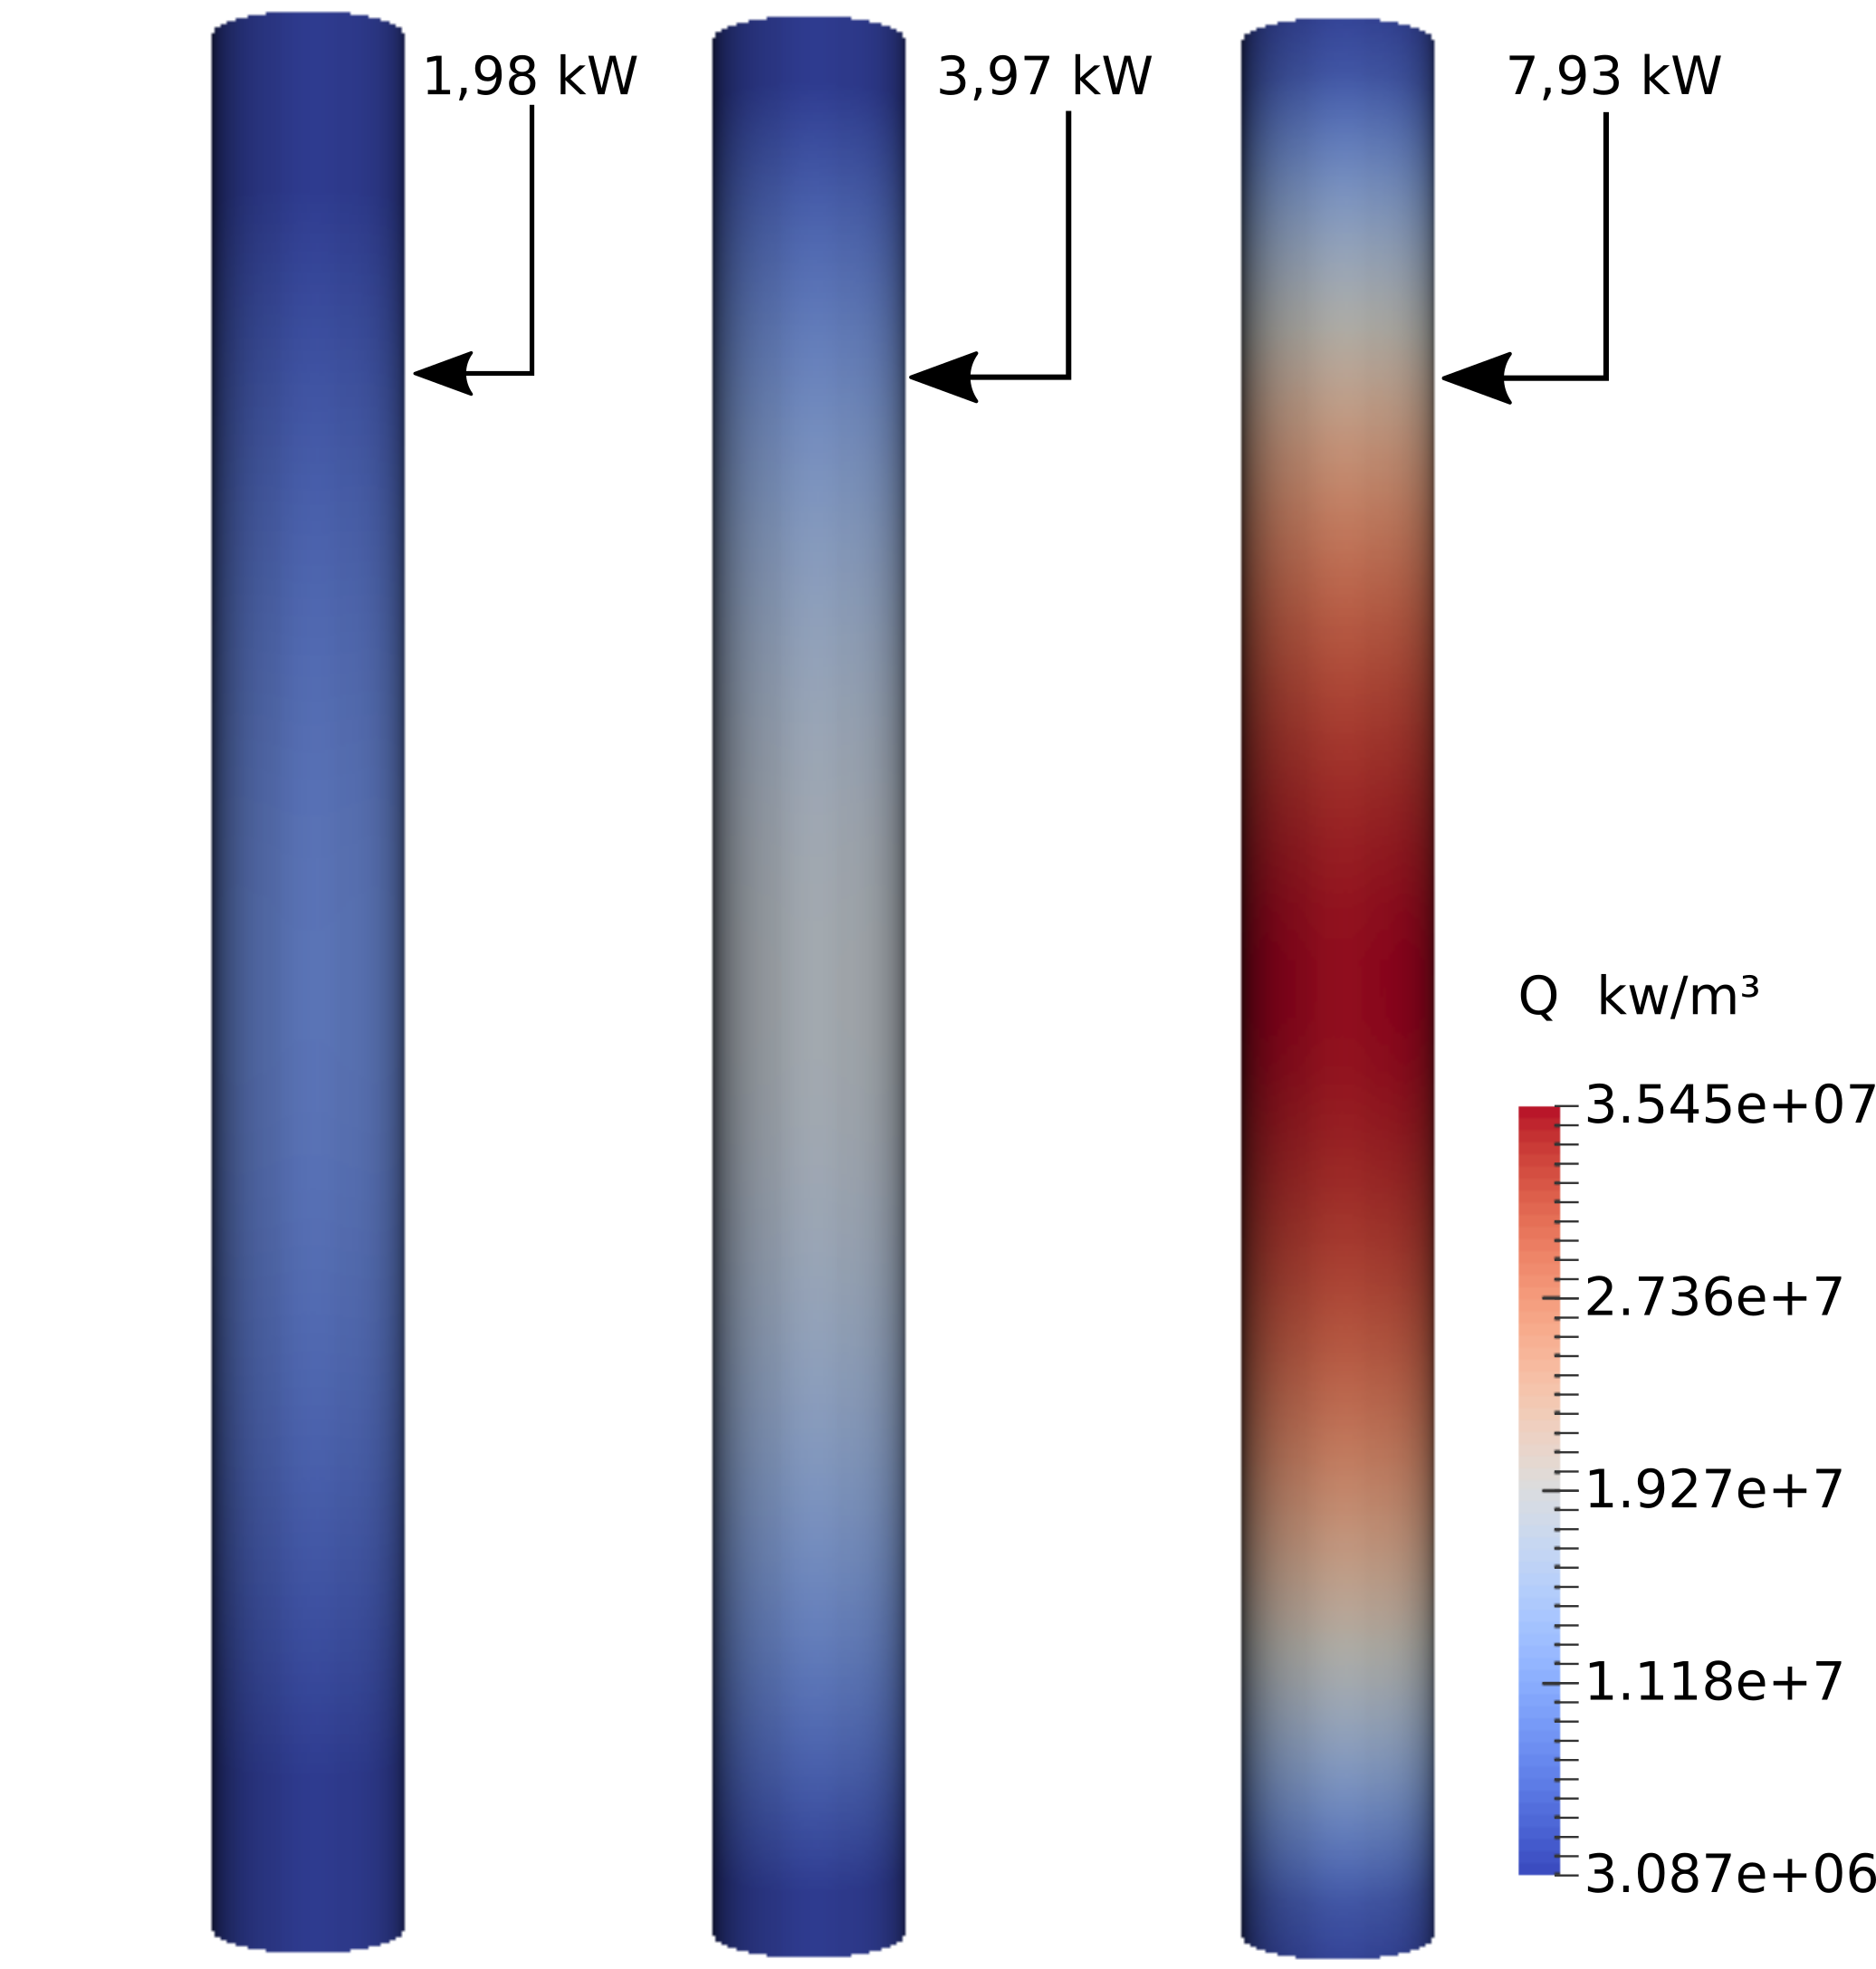
\includegraphics[scale=0.5]{figuras/Q_fuel_all_NC.png}
  \label{fig:pot-nc}
%  \legend{Fonte: autor}
\end{figure}

As distribuições de potência axial obedeceram, para os três casos, a perfis
cossenoidais, como pode ser visto na Figura \ref{fig:perf-nac-axial}. Estes são os perfis esperados para
os combustíveis modelados \cite{Veloso2005}. As distribuições de potência radiais -
obtidas do corte no ponto médio do modelo do combustível - possuem perfis diferentes
dos obtidos axialmente, como pode ser visto na Figura \ref{fig:perf-Q-nac-radial}.
A primeira e principal diferença está na abruta subida a partir da potência nula
no início e fim da curva. A razão para este comportamento é simples: apenas o combustível gera potência, sendo
zero para as regiões de revestimento e água (não apresentadas na curva). O achatamento na posição central
da curva em relação aos picos é devido ao menor fluxo térmico no centro do combustível. Nas regiões limite
entre o combustível e o revestimento, é maior o fluxo de nêutrons termalizados pela interação com o refrigerante (água).
Esse perfil é esperado em combustíveis do tipo TRIGA \cite{Ravnik1990}.

\begin{figure}[htb]
  \caption{Perfil de potência axial para os três casos simulados.}
  \centering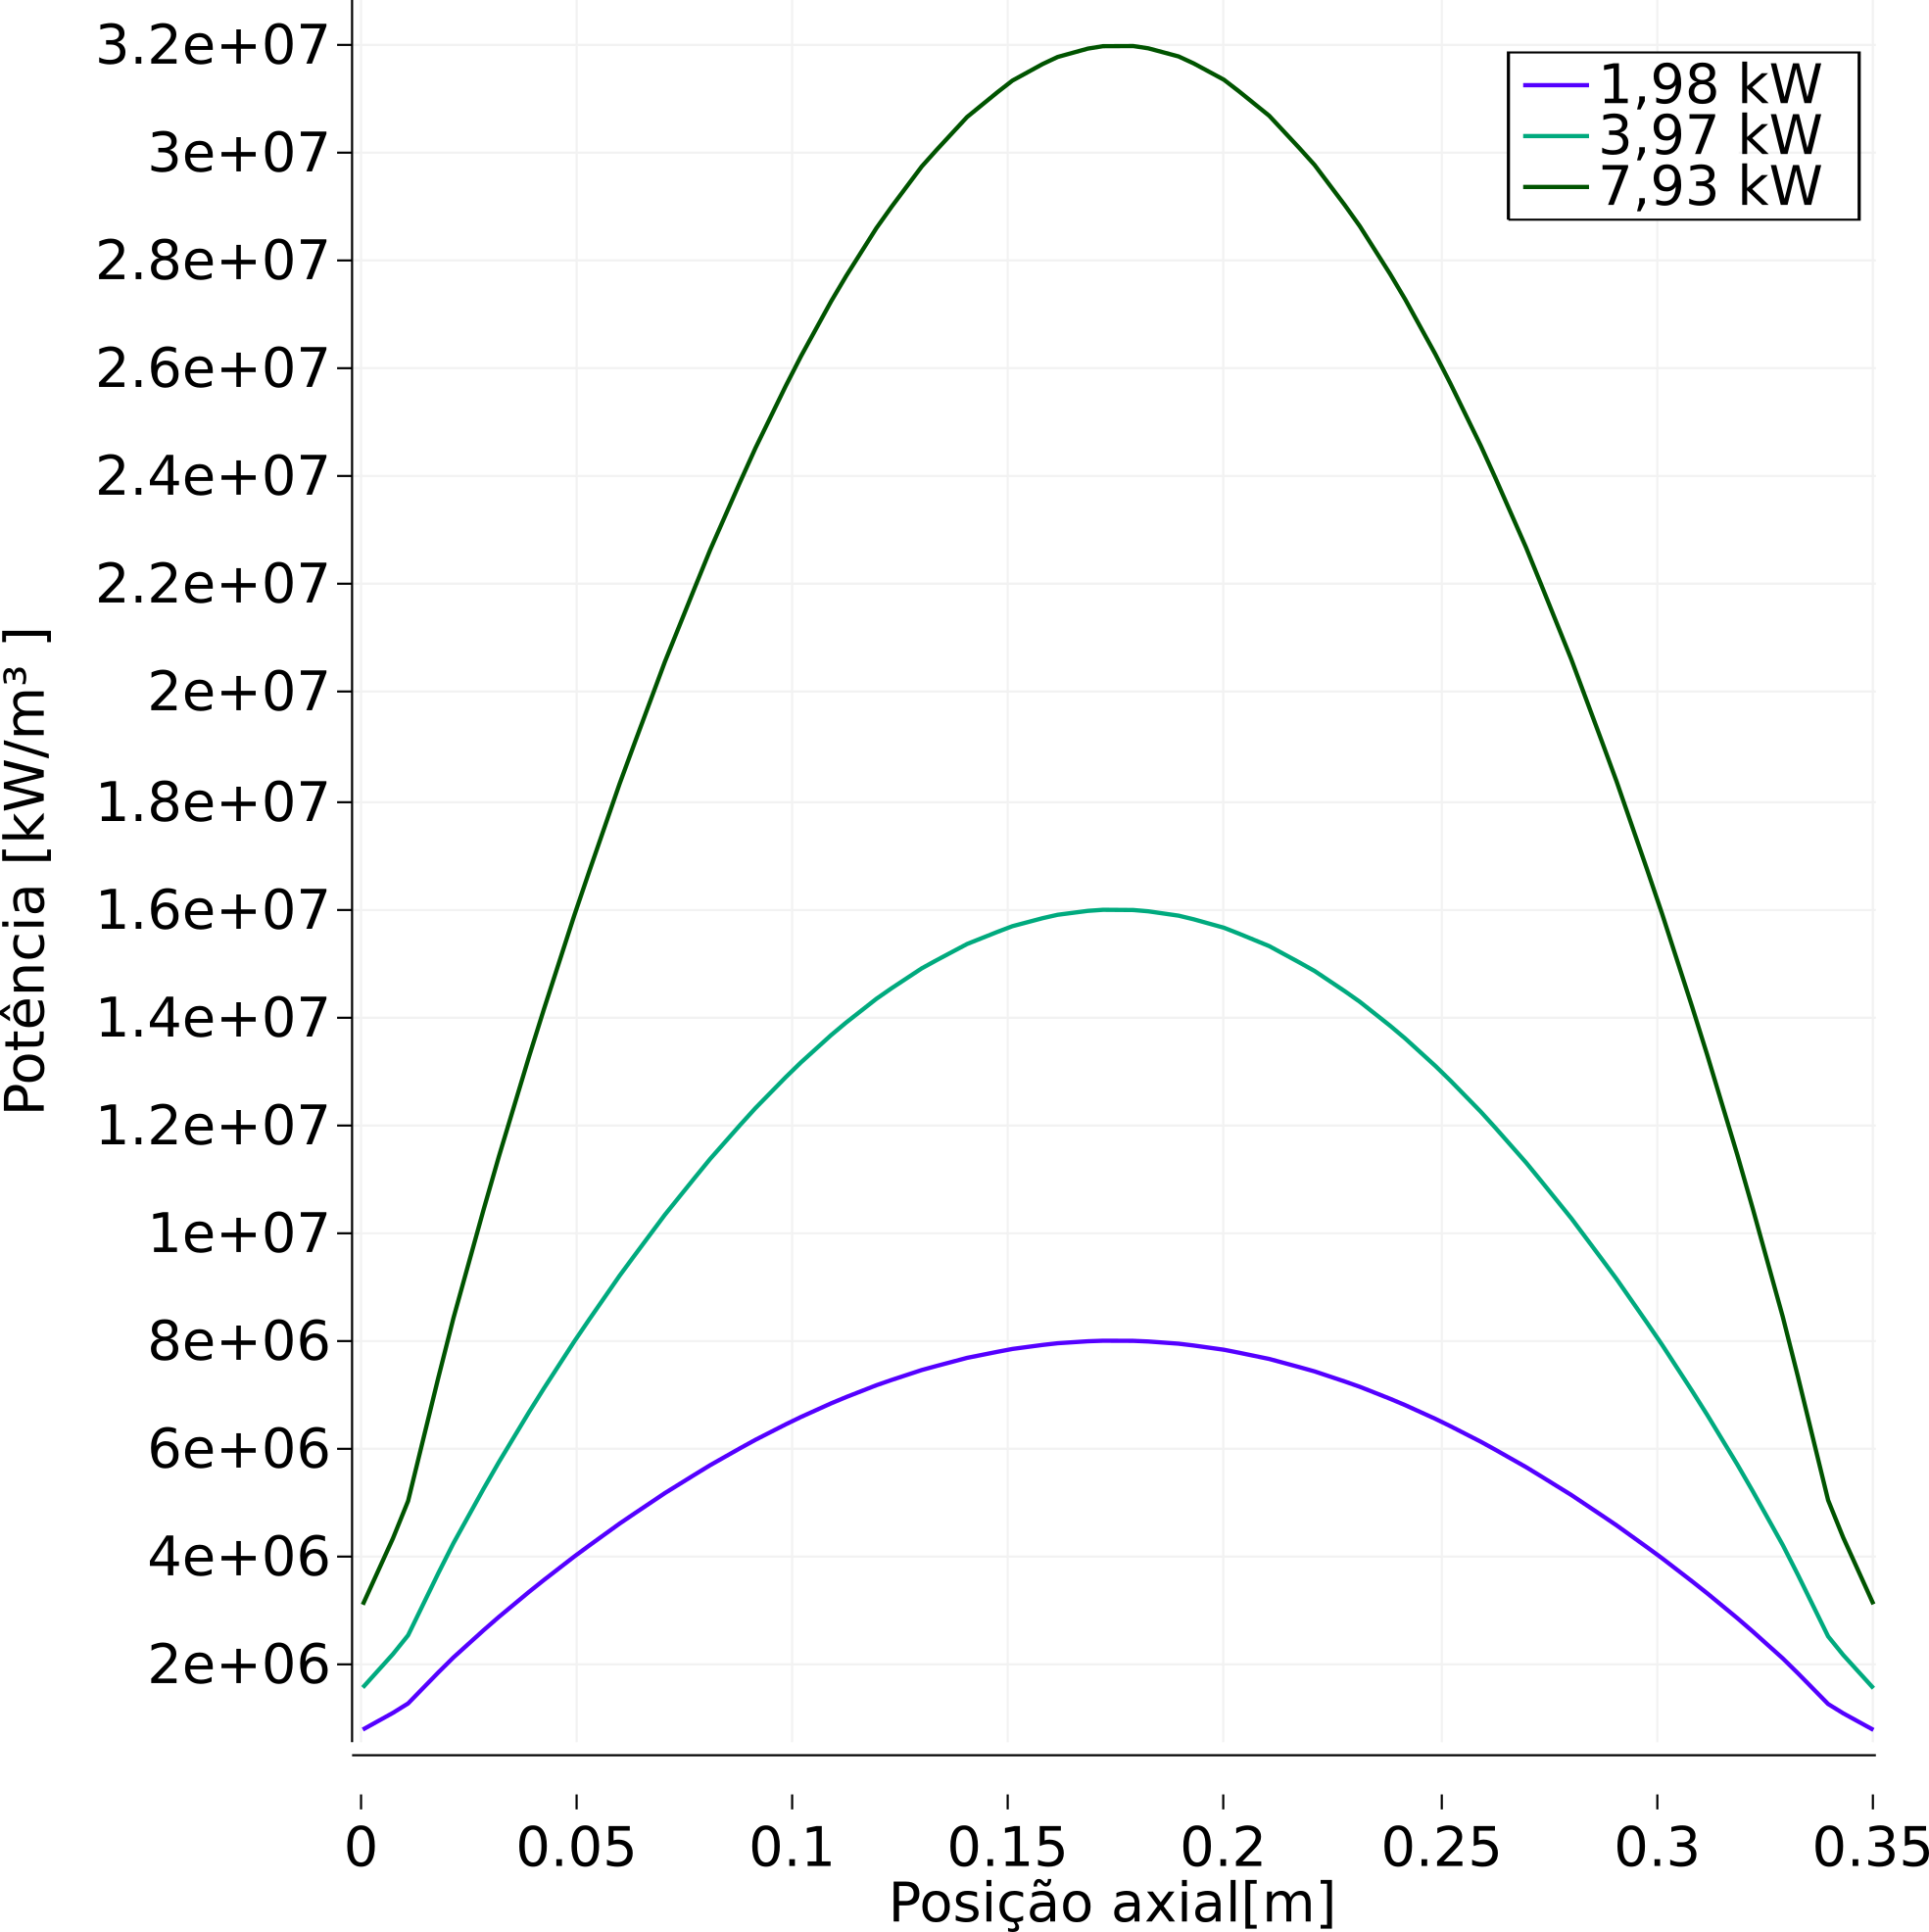
\includegraphics[scale=0.5]{figuras/Q_all_NC_port.png}
  \label{fig:perf-nac-axial}
%  \legend{Fonte: autor}
\end{figure}

\begin{figure}[htb]
  \caption[Perfil de potência radial para os três casos simulados.]{Perfil de potência radial para os três casos simulados.}
  \centering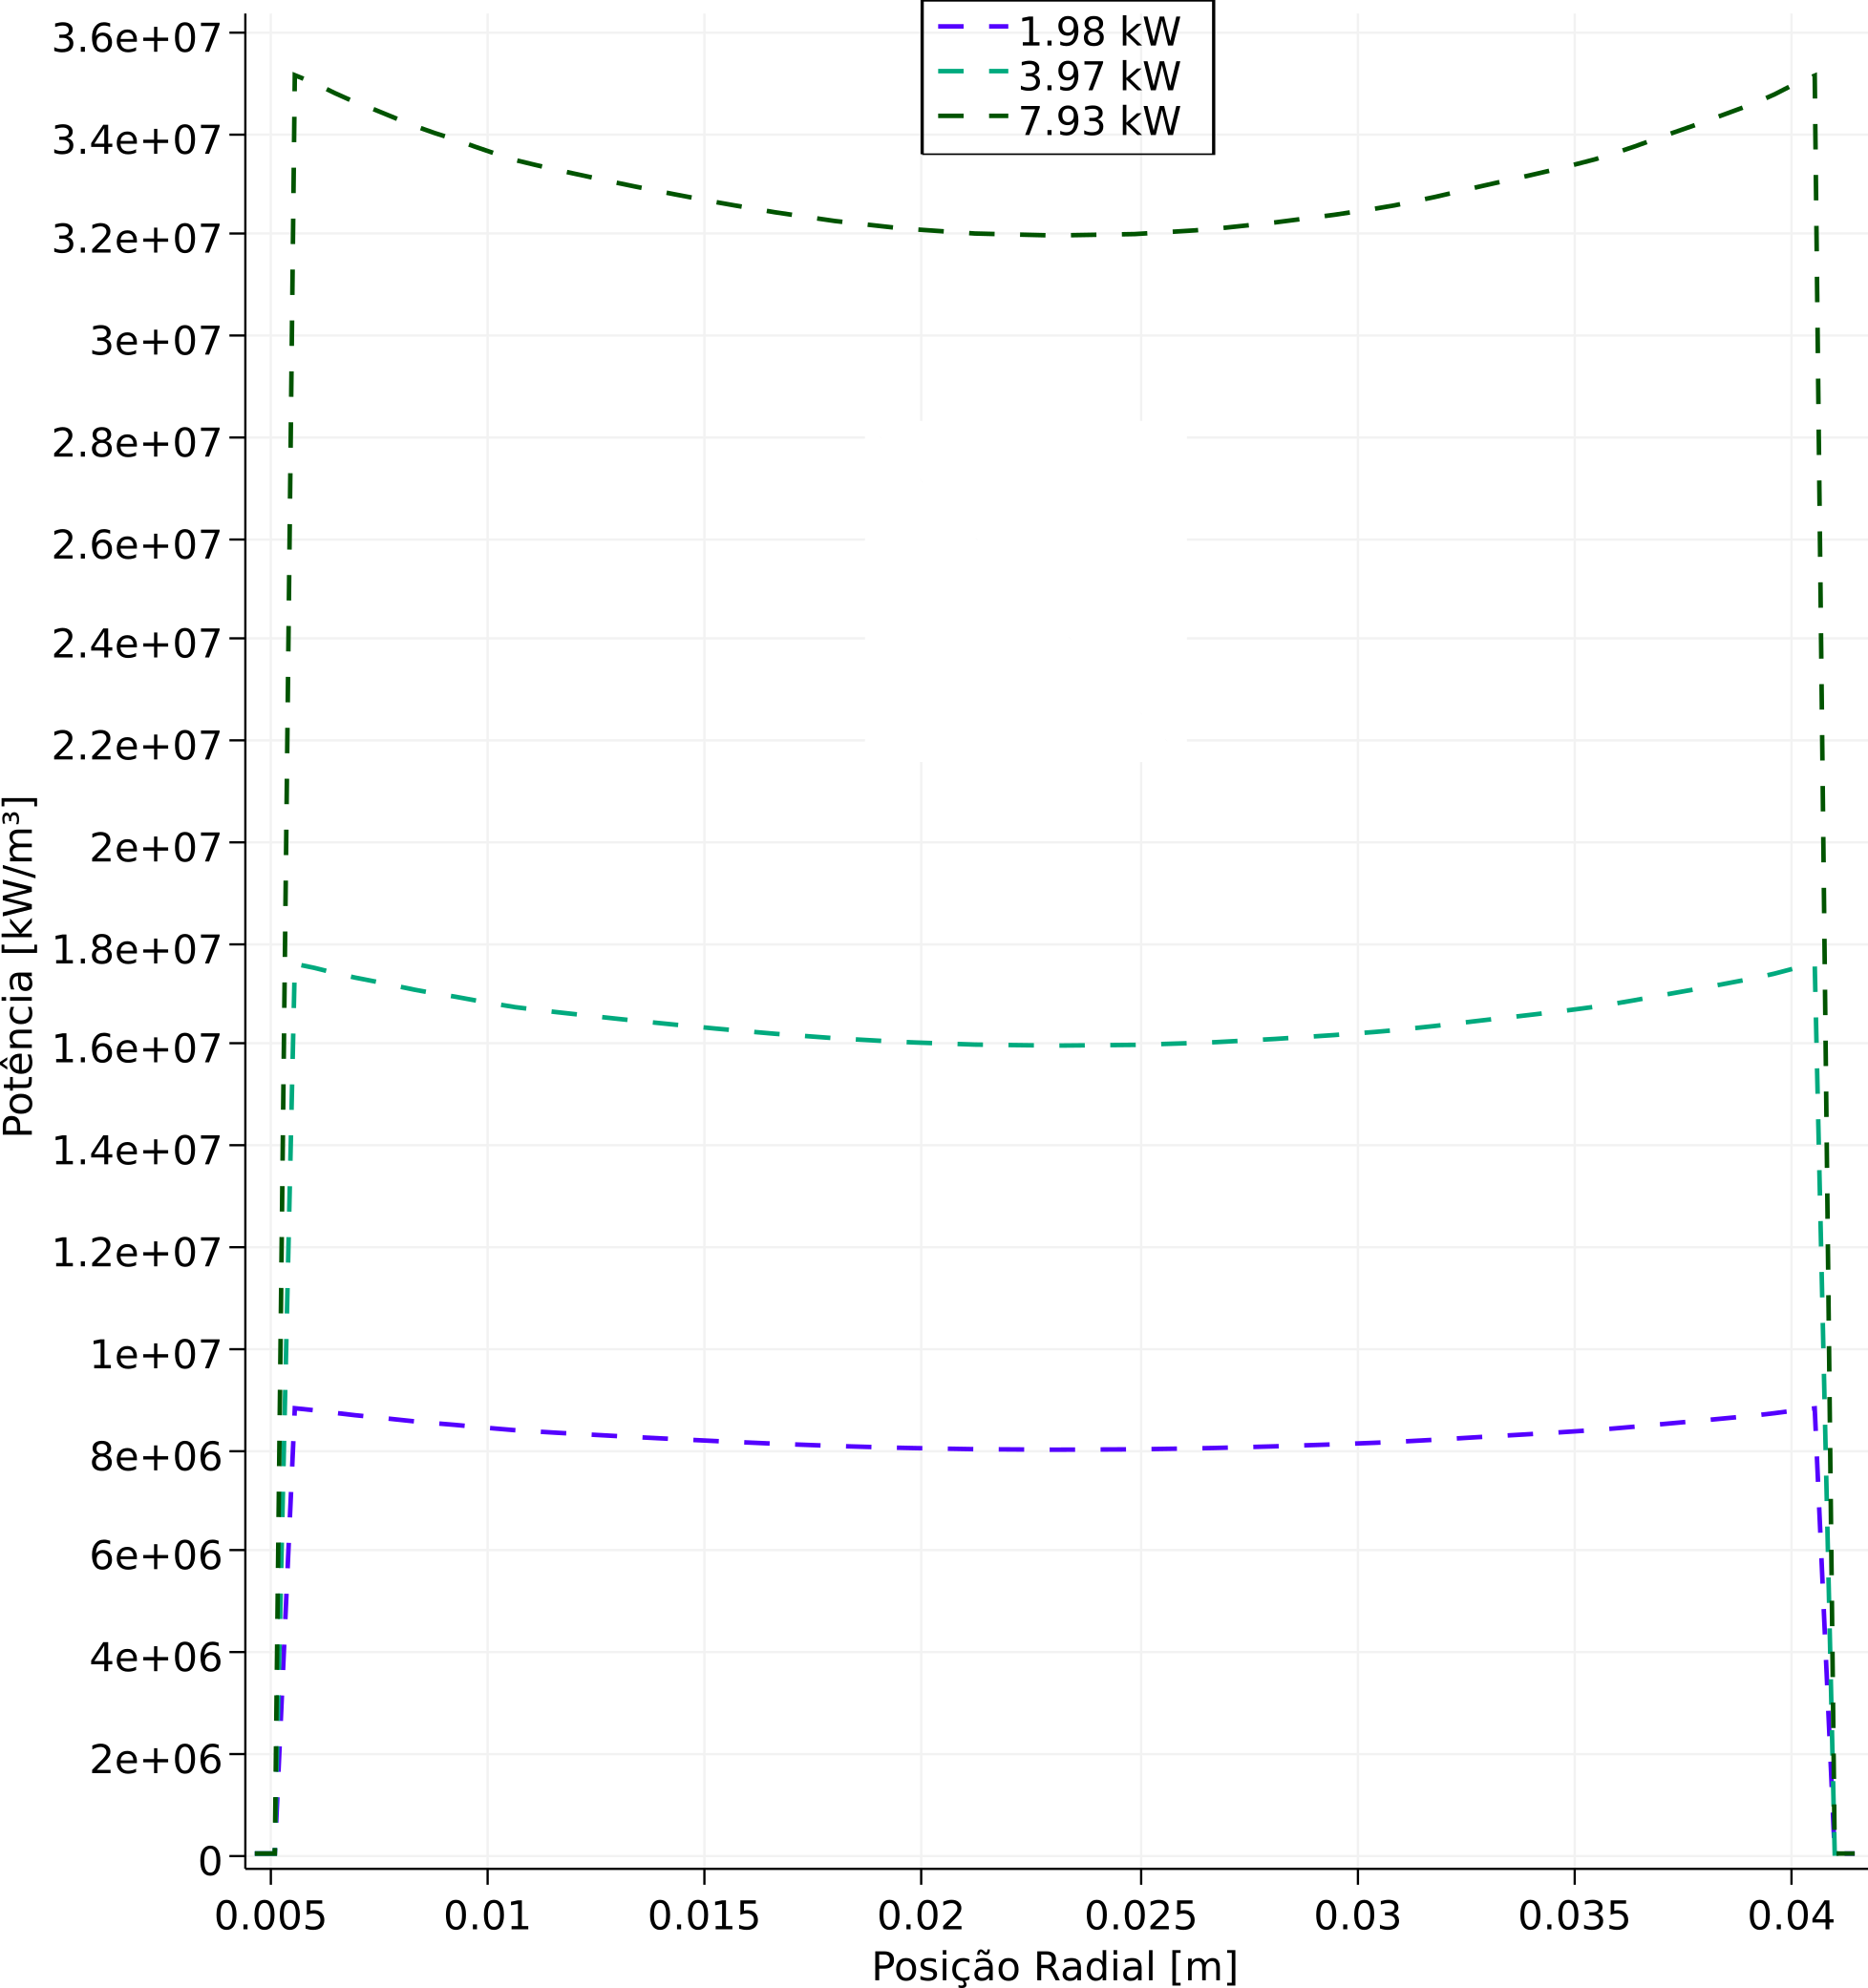
\includegraphics[scale=0.5]{figuras/Q_x_NC_square_port.png}
  \label{fig:perf-Q-nac-radial}
%  \legend{Fonte: autor}
\end{figure}

Os perfis de temperatura obtidos axialmente, Figura \ref{fig:perf-t-nac-axial},
apresentam, novamente para os três casos, uma diferença entre as extremidades
do combustível. Essa diferença é provocada pela escoamento do refrigerante (água) no
modelo. A água entra no sistema à temperatura constante de $300 K$ e, no seu trajeto,
absorve energia do sistema. Essa absorção é maior no na entrada (\textit{inlet}),
levando a uma maior resfriamento do sistema neste ponto do escoamento. Esse efeito
ocorre em todos os casos, apenas com diferença nas temperaturas de cada material.

\begin{figure}[htb]
  \caption{Perfil de temperaturas axial para os três casos simulados.}
  \centering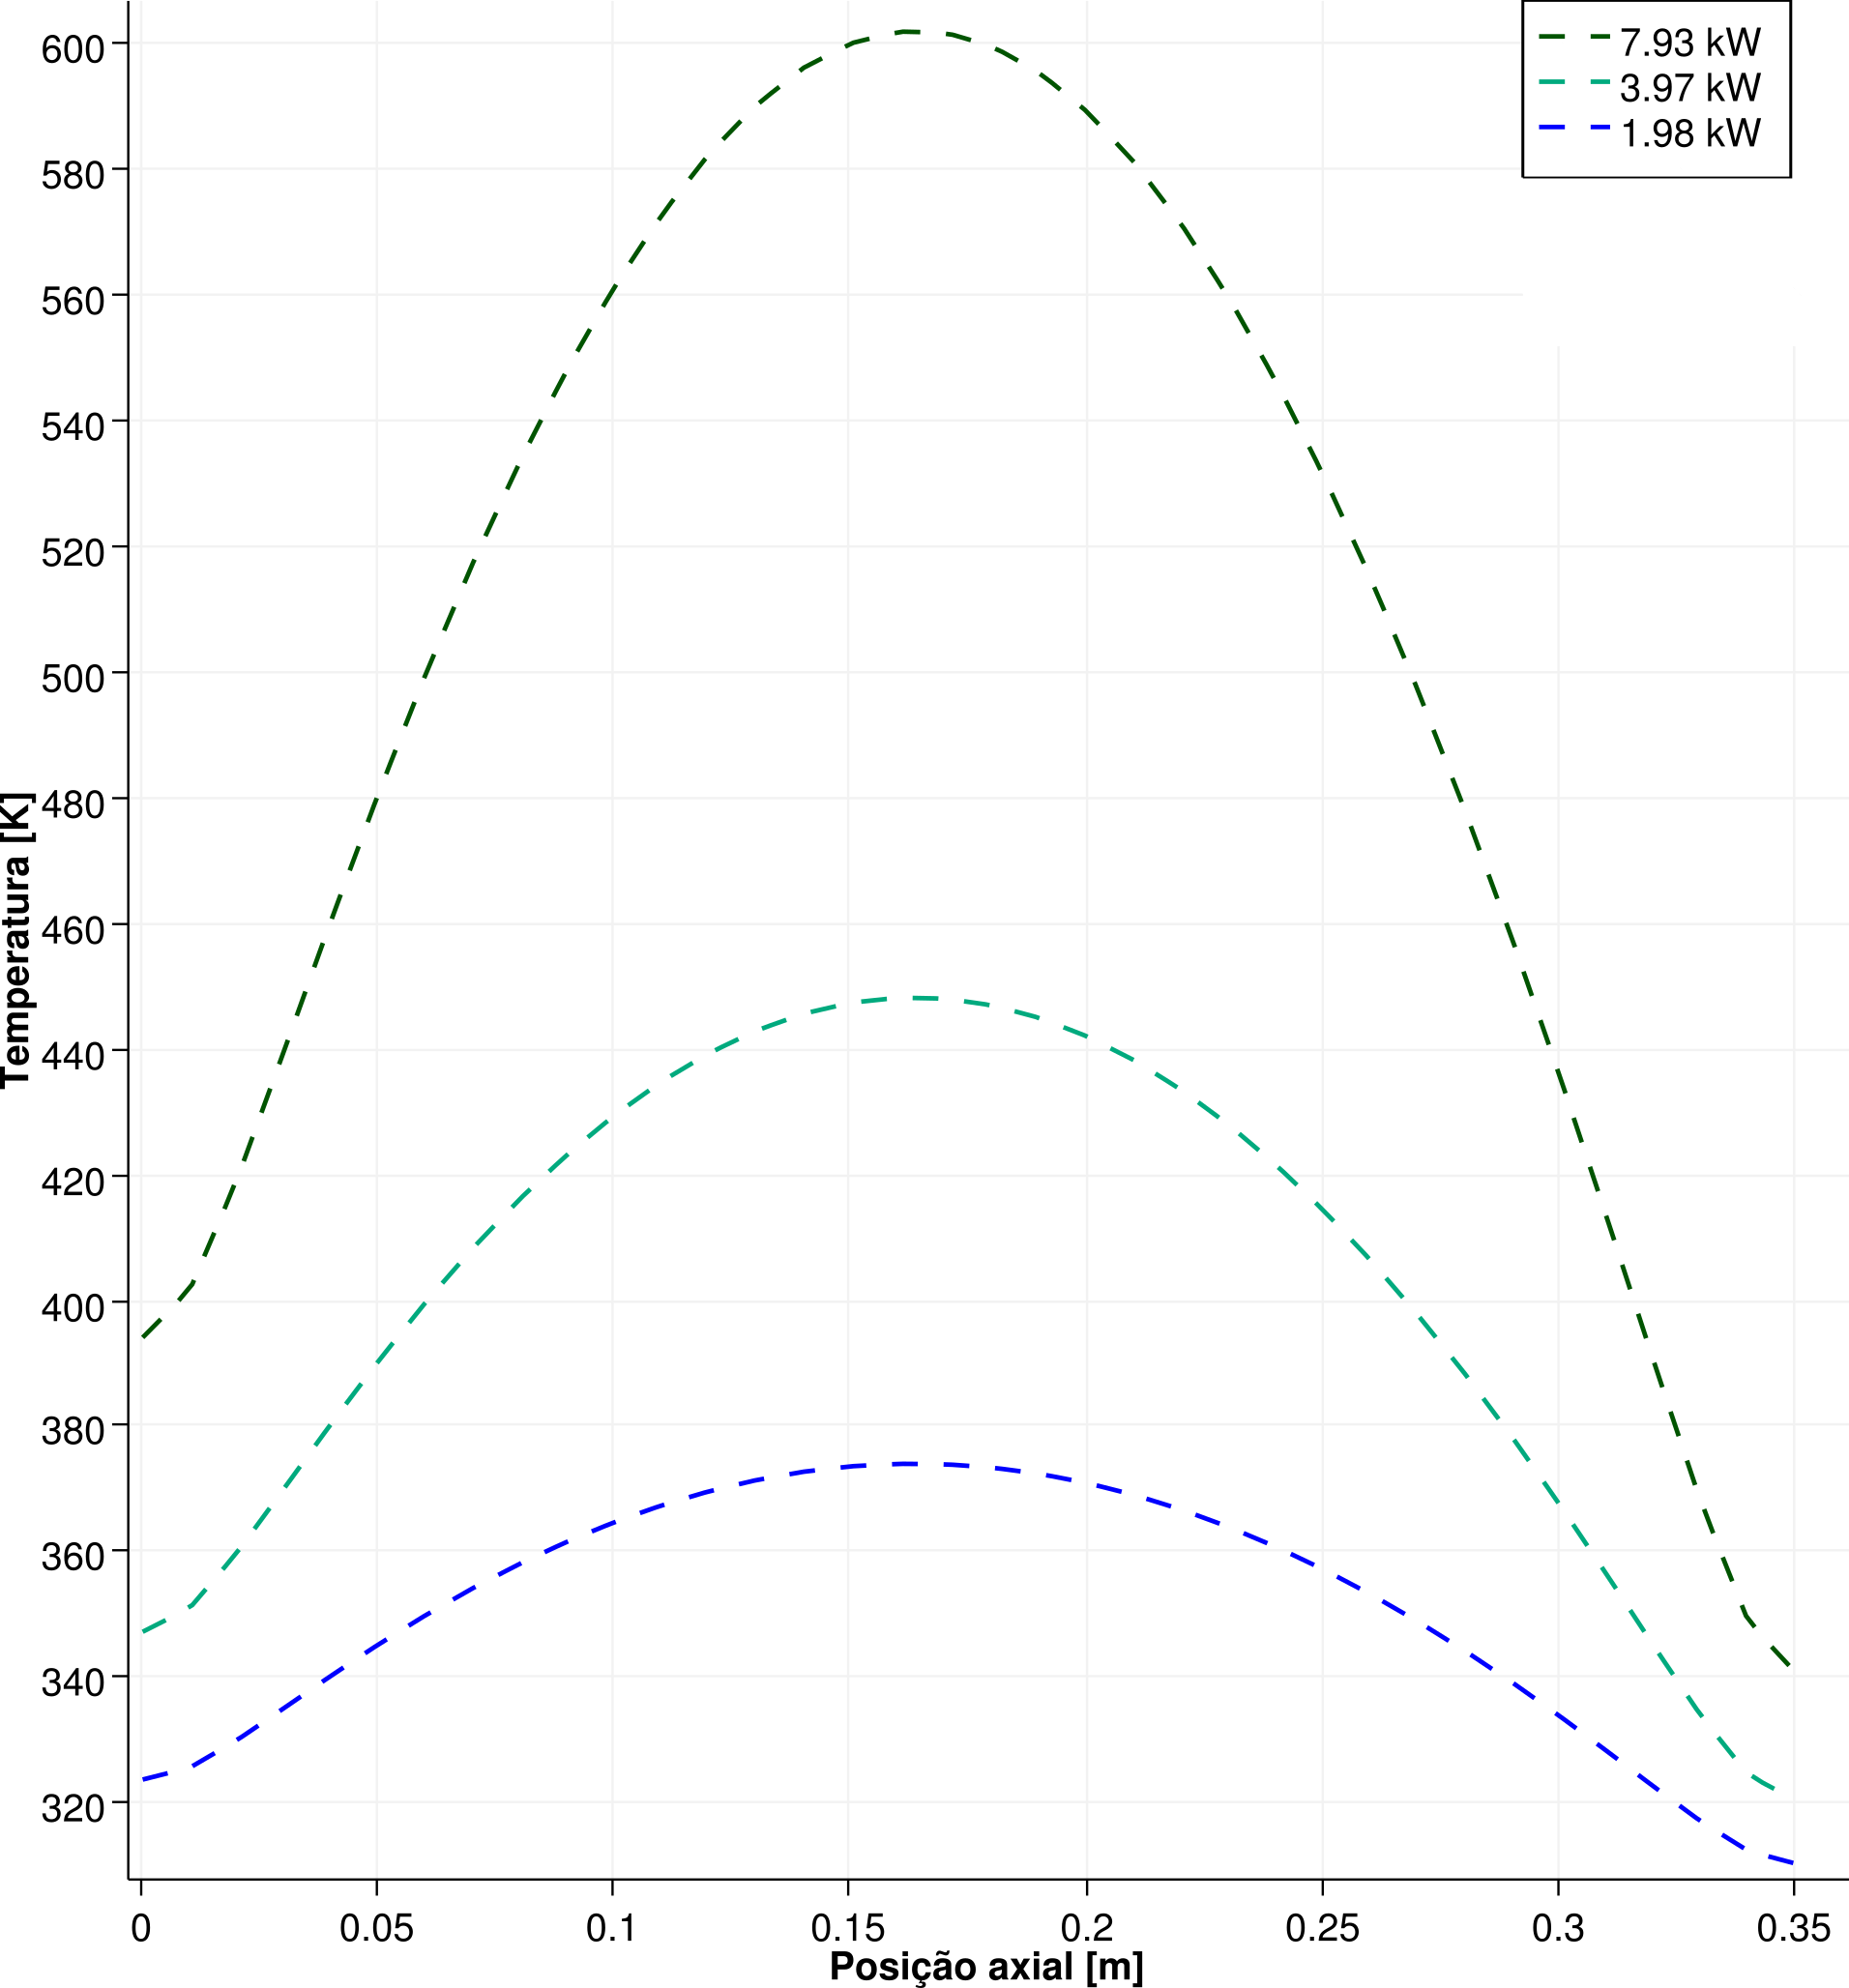
\includegraphics[scale=0.5]{figuras/T_z_NC_square_port.png}
  \label{fig:perf-t-nac-axial}
%  \legend{Fonte: autor}
\end{figure}

Radialmente, os perfis de temperatura, seguindo o mesmo padrão para os três casos simulados,
possuem descontinuidades, como pode ser visto na Figura \ref{fig:perf-t-nac-radial} (entre
$0 m$ e $0,005 m$ e $0,04 m$ e $0,045 m$). Estes degraus indicam mudança no gradiente de temperaturas na
interface entre diferentes materiais, devido às diferentes condutividades térmicas de cada um.

Os resultados das simulações apresentadas para os três casos não-acoplados formam o conjunto de resultados
de referência. Eles servem de base de comparação para as simulações acopladas, com objetivo de verificar
se os resultados acoplados se diferenciam destes e em que medida ocorrem estas diferenças.

\begin{figure}[htb]
  \caption[Perfil de temperaturas radial para os três casos simulados.]
          {Perfil de temperaturas radial para os três casos simulados. No detalhe o perfil de temperatura nas interfaces entre os três materiais.}
  \centering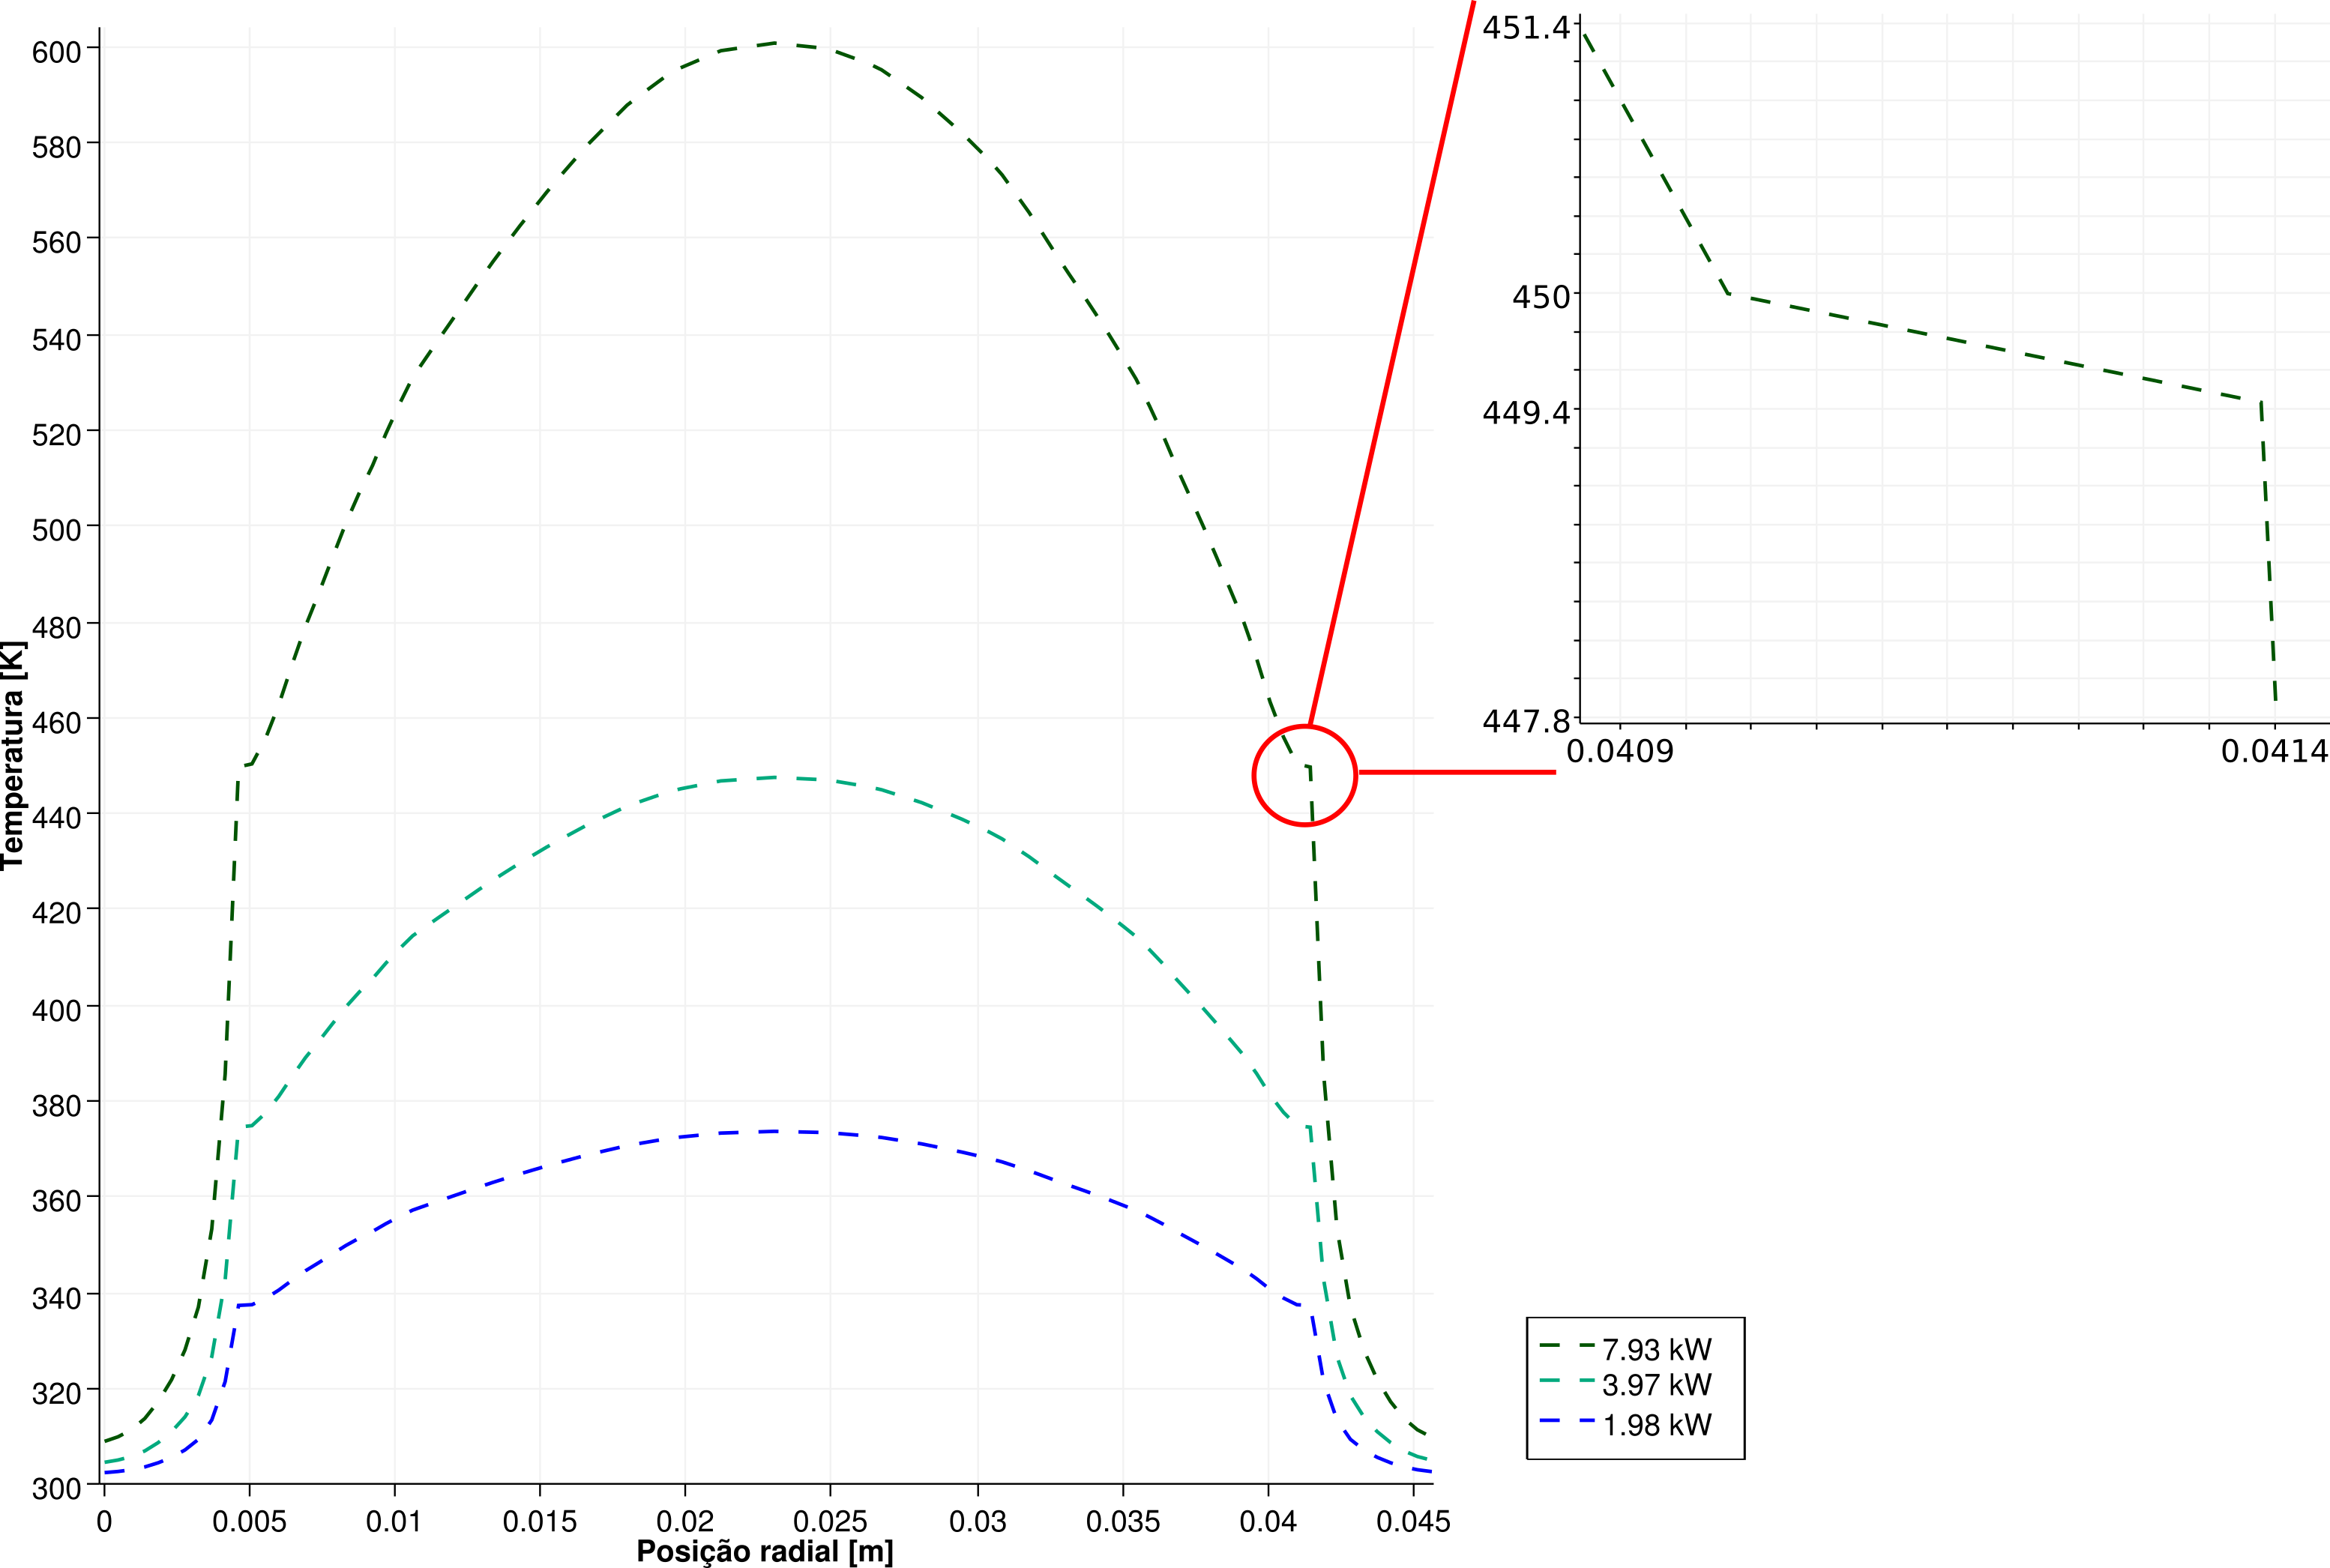
\includegraphics[scale=0.5]{figuras/T_x_NC_square_port_detalhado.png}
  \label{fig:perf-t-nac-radial}
%  \legend{Fonte: autor}
\end{figure}


% ------------------------------------------------------------------------------------------------------------
\section{Caso acoplado}
\label{sec:cp}

As simulações acopladas foram realizadas exatamente nas mesmas condições das suas homólogas não-acopladas.
Os resultados destas são apresentados em comparação com os resultados de referência para visualização
das diferenças entre elas.

Diferentemente dos cálculos não-acoplados, na simulação acoplada ocorre a variação do fluxo neutrônico.
Essa variação, originada da variação de temperaturas no sistema, ocorre nos três casos acoplados, cada
um simulado numa potência.

Para as simulações a $1,98 kW$, as diferenças no fluxo são as mais sutis. Com potência mais baixa, há menor
diferença nas temperaturas entre o caso acoplado e o não-acoplado. Como as seções de choque variam de
acordo com a temperatura, é menor a diferença entre seções de choque. Por consequência, menor a diferença
no fluxo neutrônico. Outro fator que leva à similaridade entre os fluxos é a baixa granularidade
da malha na direção axial (apenas 35 camadas de elementos, como apresentado na Tabela \ref{tab:size_model}).

Na Figura \ref{fig:flux_z_50} são apresentados os fluxos axiais acoplados e não acoplados nas simulações
à potência mais baixa, de $1,98 kW$. A diferença entre os fluxos é melhor percebida no corte radial,
apresentado na Figura \ref{fig:flux_x_50}. Além de uma maior variação radial devido à moderação de nêutrons
nas paredes, e consequente aumento do fluxo térmico, a malha é mais refinada radialmente. Com isso, é possível
captar mais detalhes do fluxo neutrônico.

%Ver se dá pra colocar tempo e parâmetros de convergência.

\begin{figure}[htb]
  \caption{Fluxos relativos axiais entre simulação acoplada e não acoplada para
    potência de 1,98 kW.}
  \centering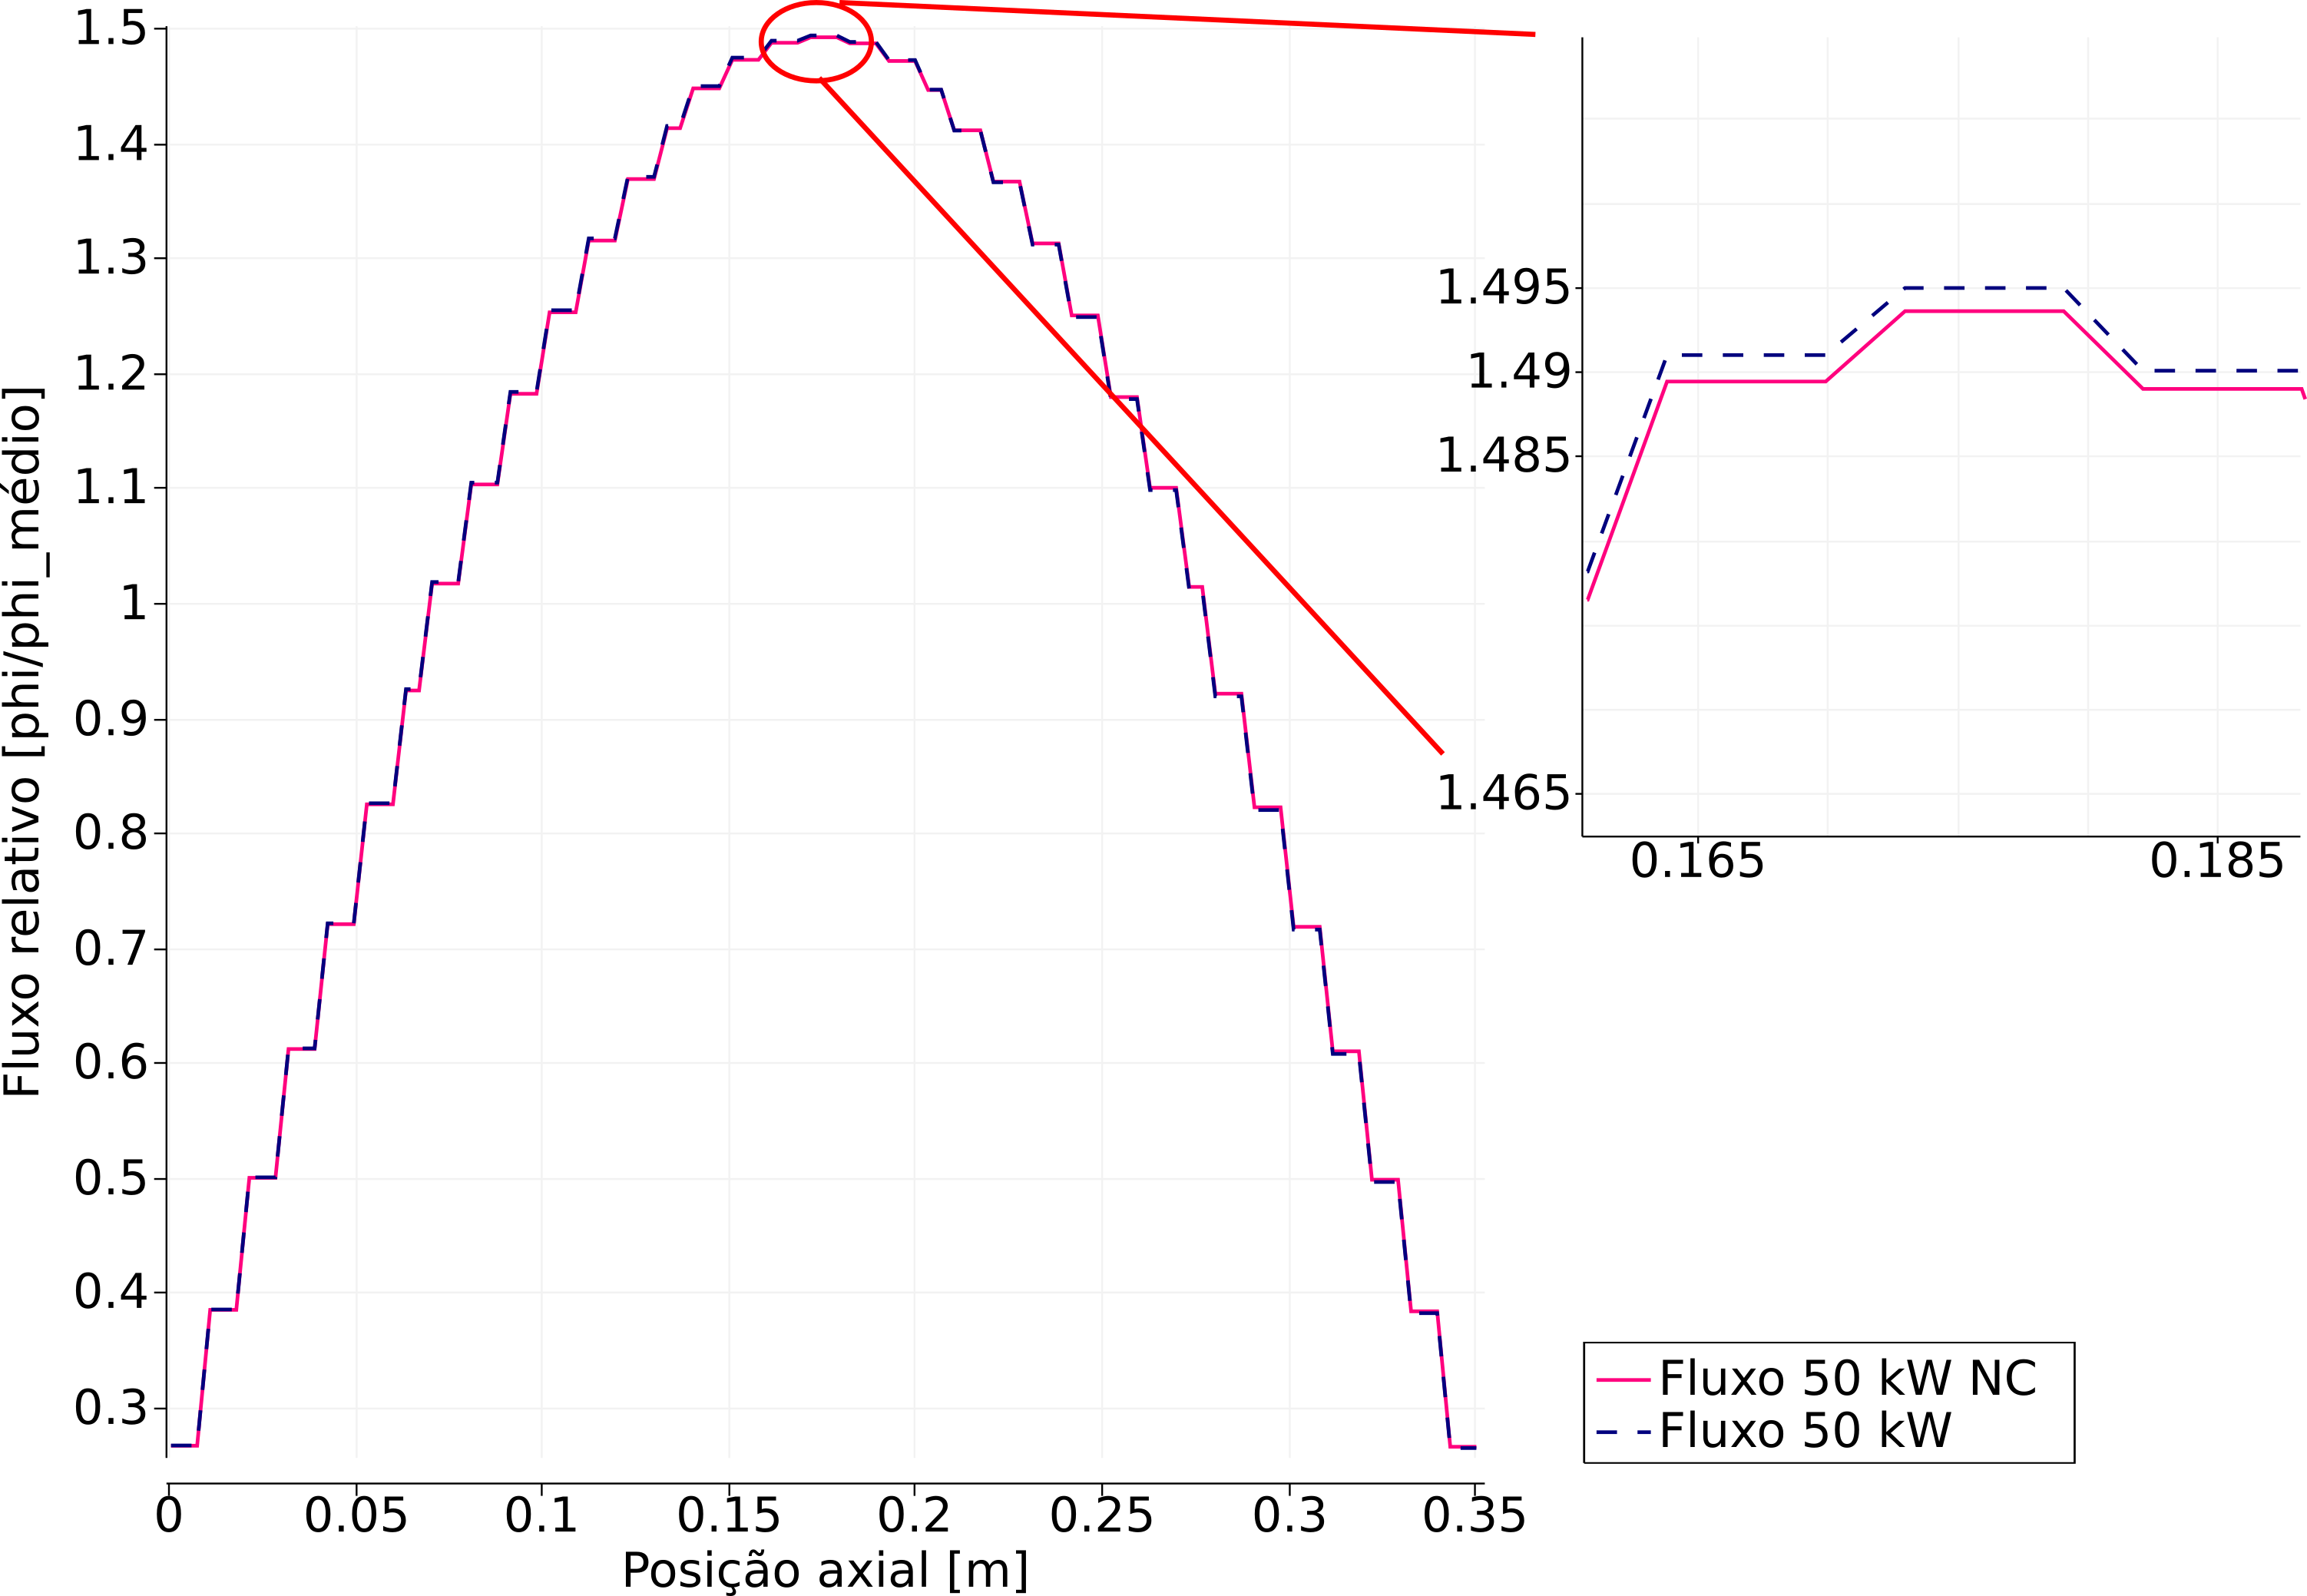
\includegraphics[scale=0.5]{figuras/Flux_rel_z_50_port_trabalhado.png}
  \label{fig:flux_z_50}
%  \legend{Fonte: autor}
\end{figure}

\begin{figure}[htb]
  \caption{Fluxos relativos radiais entre simulação acoplada e não acoplada para
    potência de 1,98 kW.}
  \centering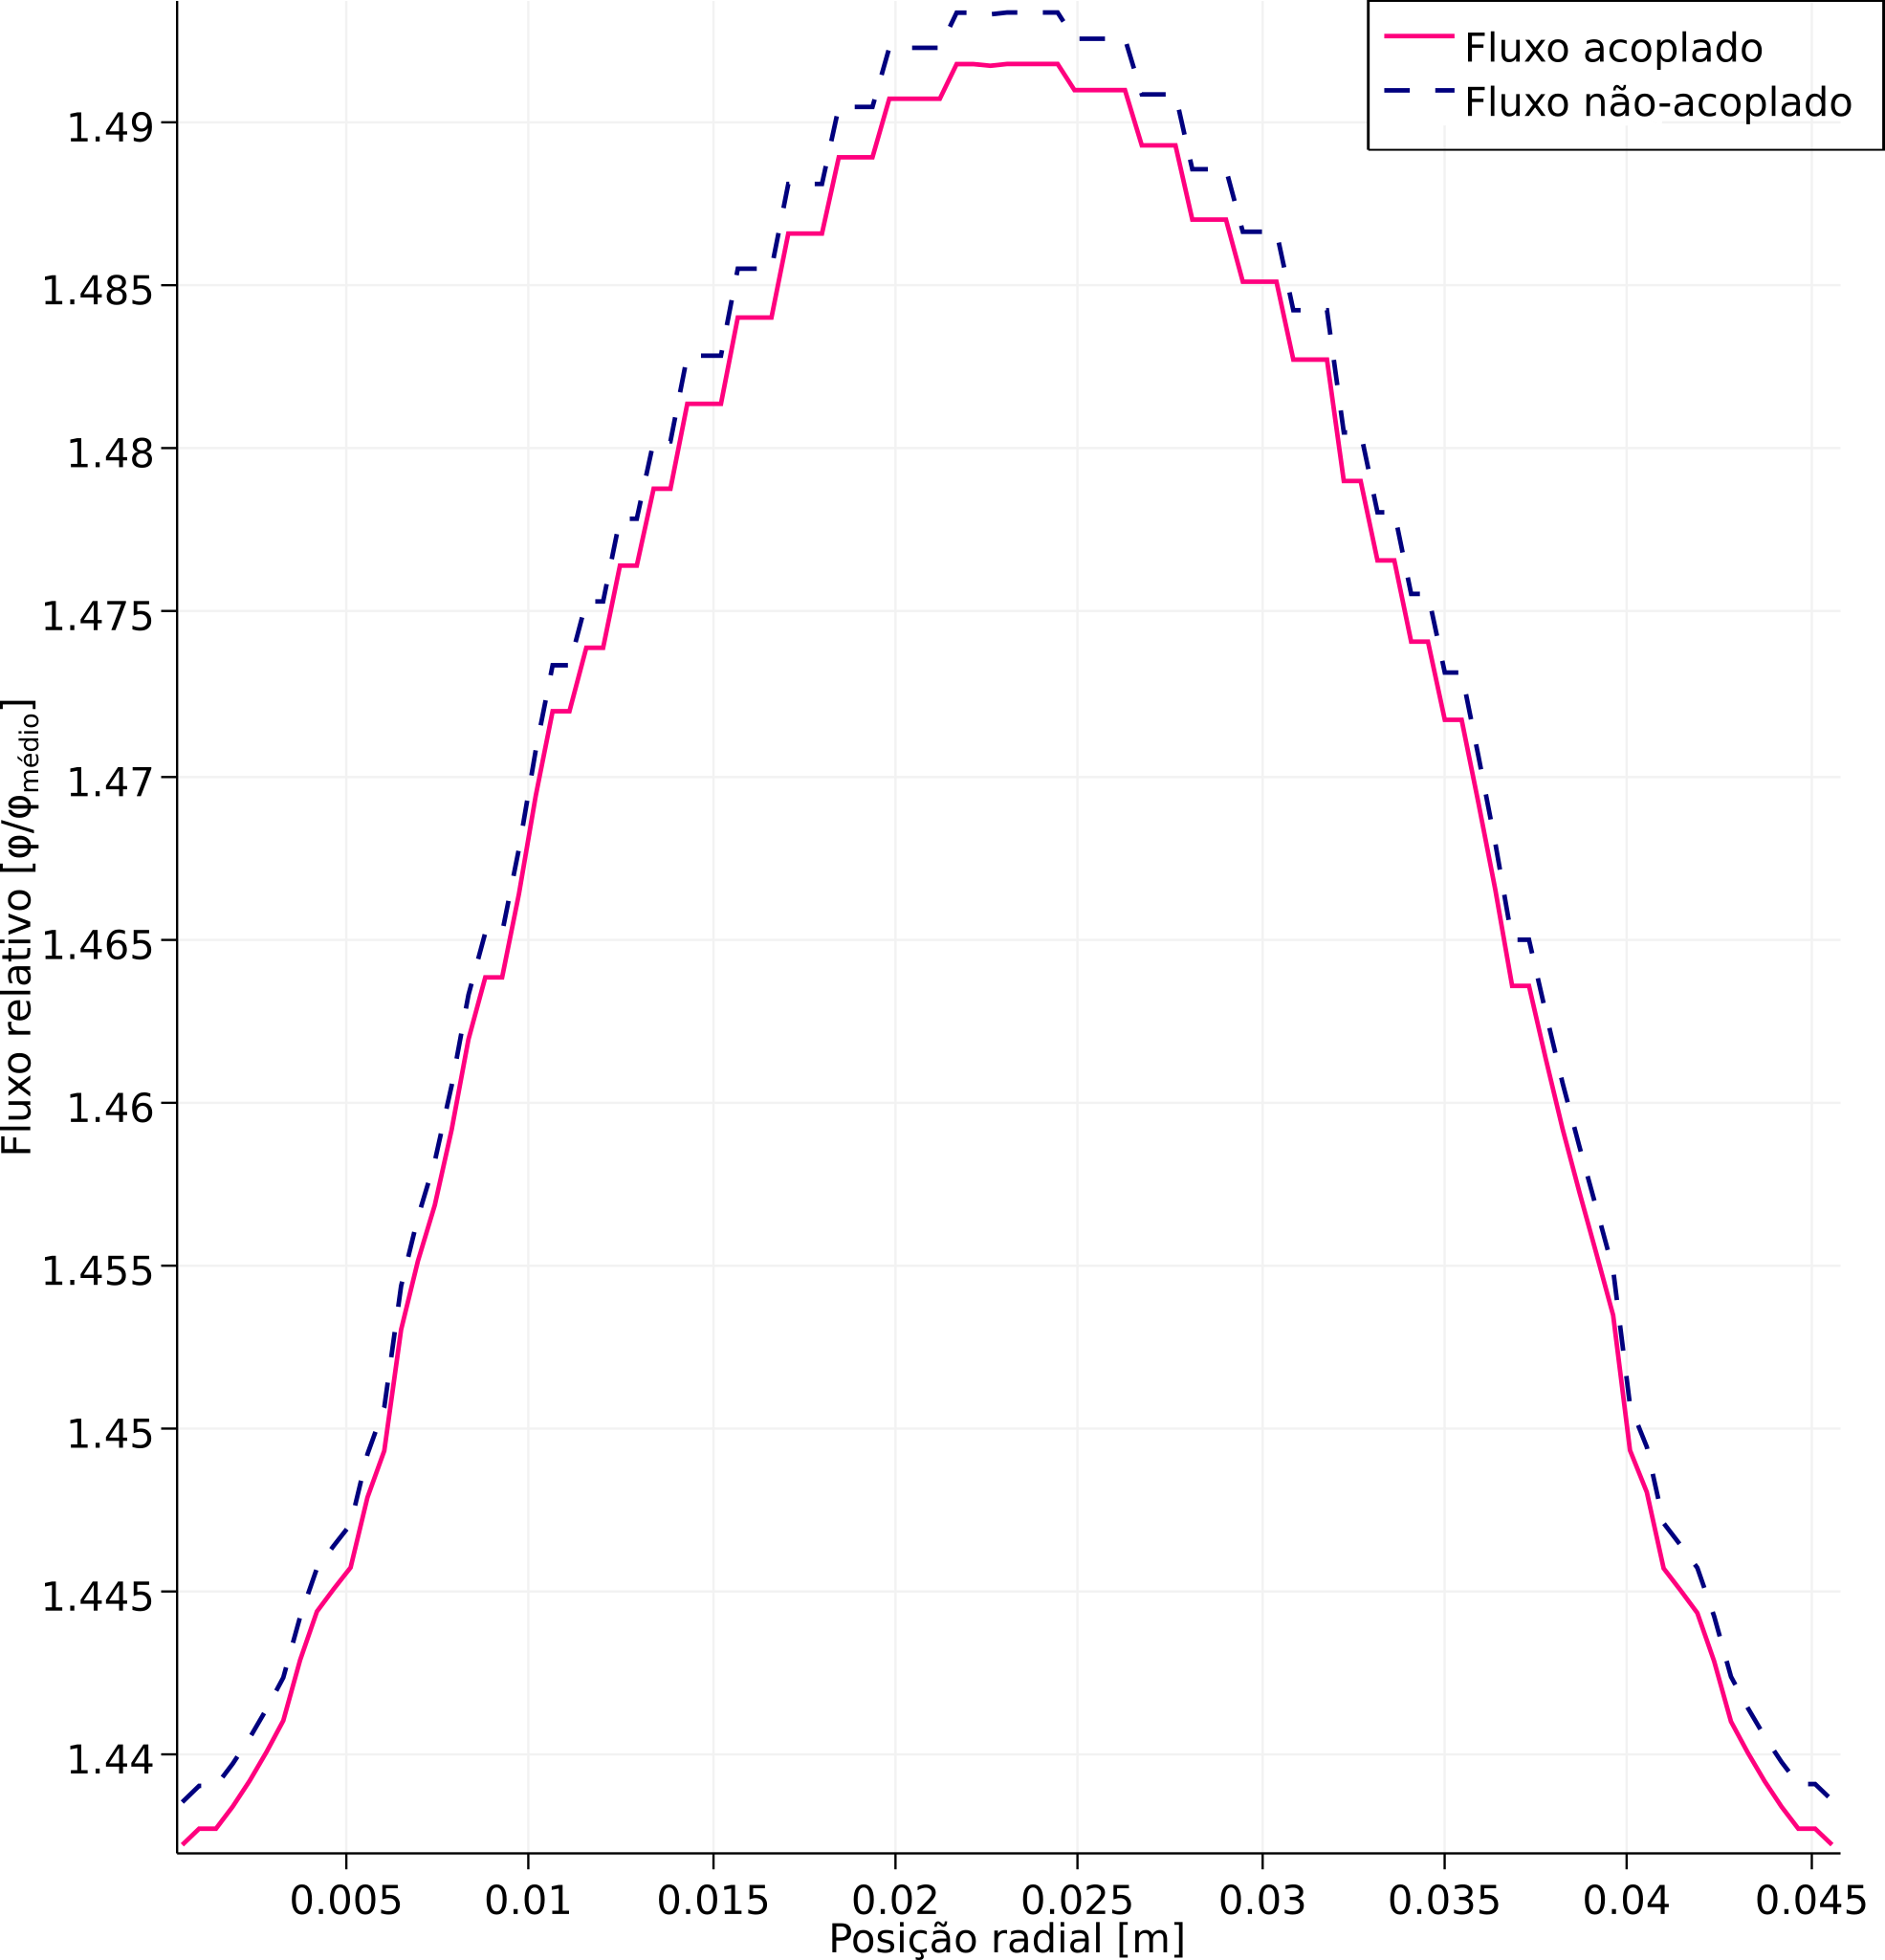
\includegraphics[scale=0.5]{figuras/Flux_rel_x_50_port.png}
  \label{fig:flux_x_50}
%  \legend{Fonte: autor}
\end{figure}

As mesmas observações feitas para os fluxos relativos na menor potência são válidas
para as simulações feitas à potência de $3,97 kW$. Novamente, as diferenças entre
os fluxos relativos são melhor observáveis no corte radial do que no corte axial.
Entretanto, as diferenças entre os fluxo começam a aumentar de acordo com o
aumento da potência. Os fluxos relativos axiais acoplados e não-acoplados para
potência de $3,97 kW$ podem ser observados na Figura \ref{fig:flux_z_100}, enquanto
os fluxos relativos radiais para a mesma potência podem ser observados na Figura \ref{fig:flux_x_100}.

\begin{figure}[htb]
  \caption{Fluxos relativos axiais entre simulação acoplada e não acoplada para
    potência de 3,97 kW.}
  \centering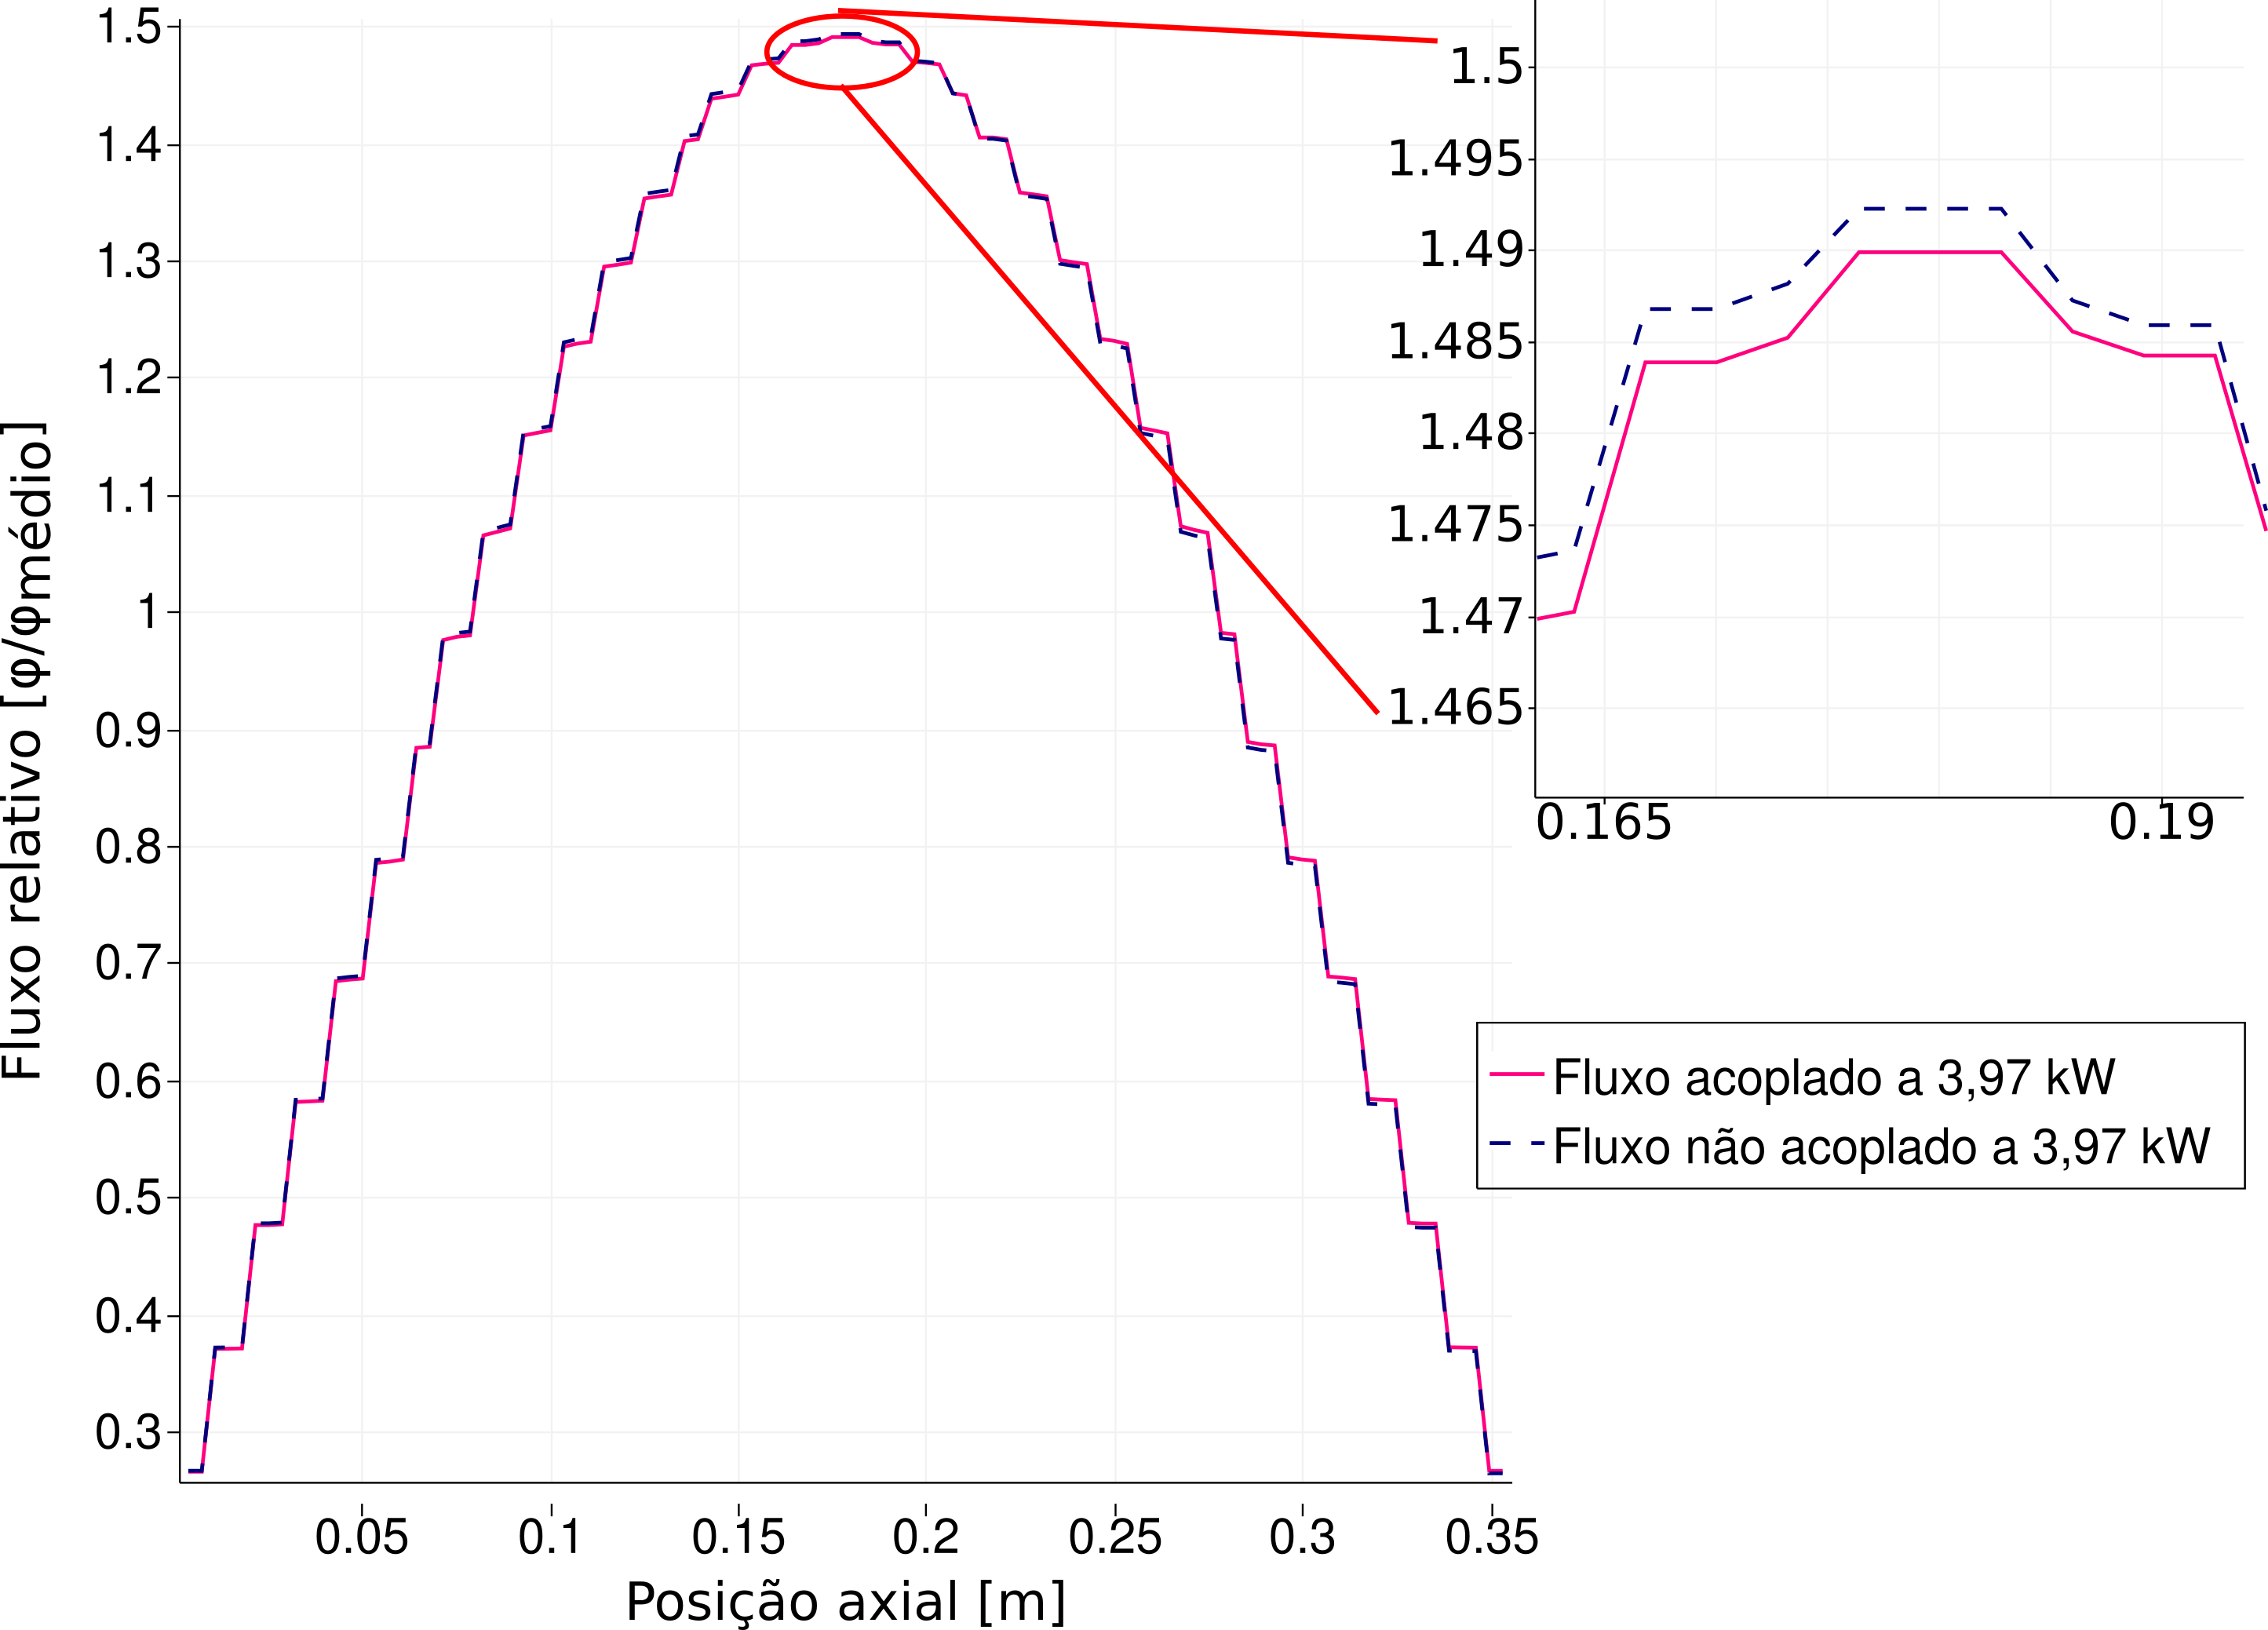
\includegraphics[scale=0.5]{figuras/Flux_rel_z_100_port_trabalhado.png}
  \label{fig:flux_z_100}
%  \legend{Fonte: autor}
\end{figure}

\begin{figure}[htb]
  \caption{Fluxos relativos radiais entre simulação acoplada e não acoplada para
    potência de 3,97 kW.}
  \centering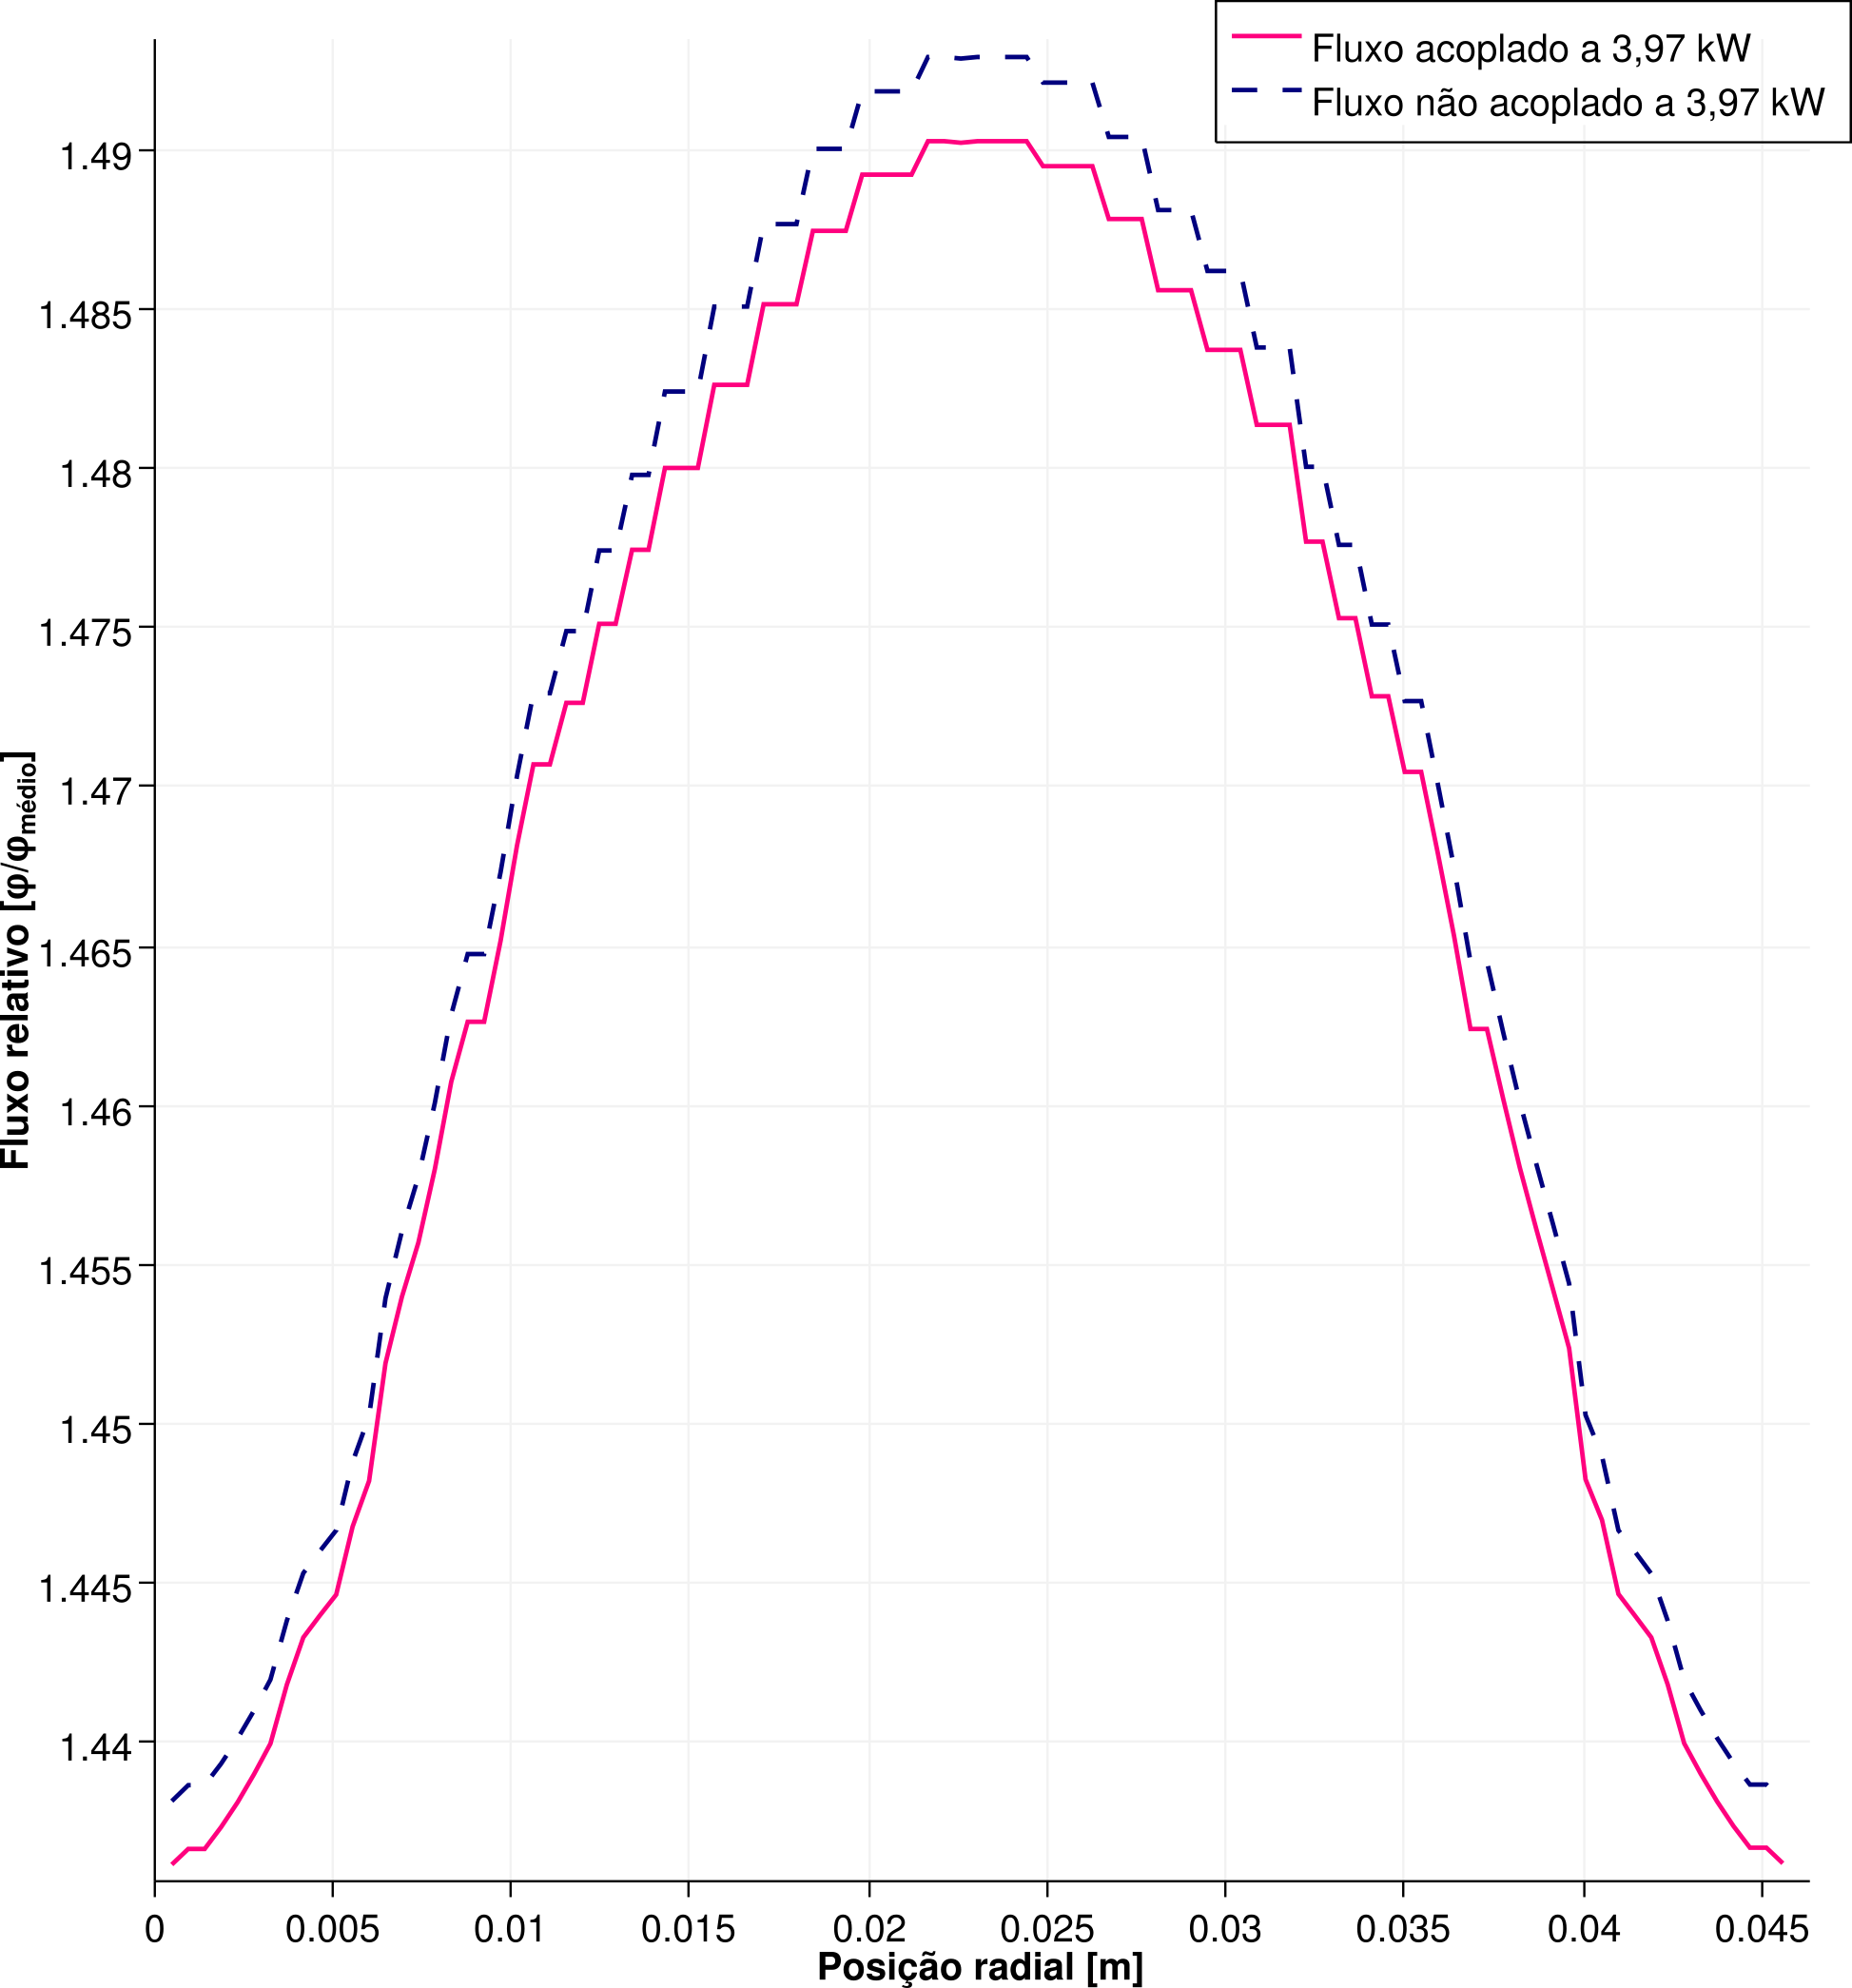
\includegraphics[scale=0.5]{figuras/Flux_rel_x_100_port.png}
  \label{fig:flux_x_100}
%  \legend{Fonte: autor}
\end{figure}

As diferenças entre os fluxos relativos em ambas as simulações passa a ser melhor
vista nas simulações de maior potência, a $7,93 kW$. Novamente, a variação nas temperaturas
impacta nos cálculos acoplados, uma vez que as seções de choque são periodicamente
ajustadas. É possível observar na Figura \ref{fig:flux_z_200}, que apresenta o perfil axial,
uma sutil sobreposição entre as curvas, demonstrando um achatamento na curva
referente as cálculos acoplados. Isso se explica pelas propriedades do combustível modelado,
que diminui sua capacidade de absorção de nêutrons térmicos com o aumento da temperatura.
Ao mesmo tempo, nas extremidades da curva, as temperaturas são menores que no caso não-acoplado,
levando a um relativo aumento no fluxo. O fluxo acoplado reflete tais mudanças no seu perfil.

As diferenças entre os fluxos relativos radiais, para a potência de $7,93 kW$, são facilmente
visíveis na Figura \ref{fig:flux_x_200}.

\begin{figure}[htb]
  \caption{Fluxos relativos axiais entre simulação acoplada e não acoplada para
    potência de 7,93 kW.}
  \centering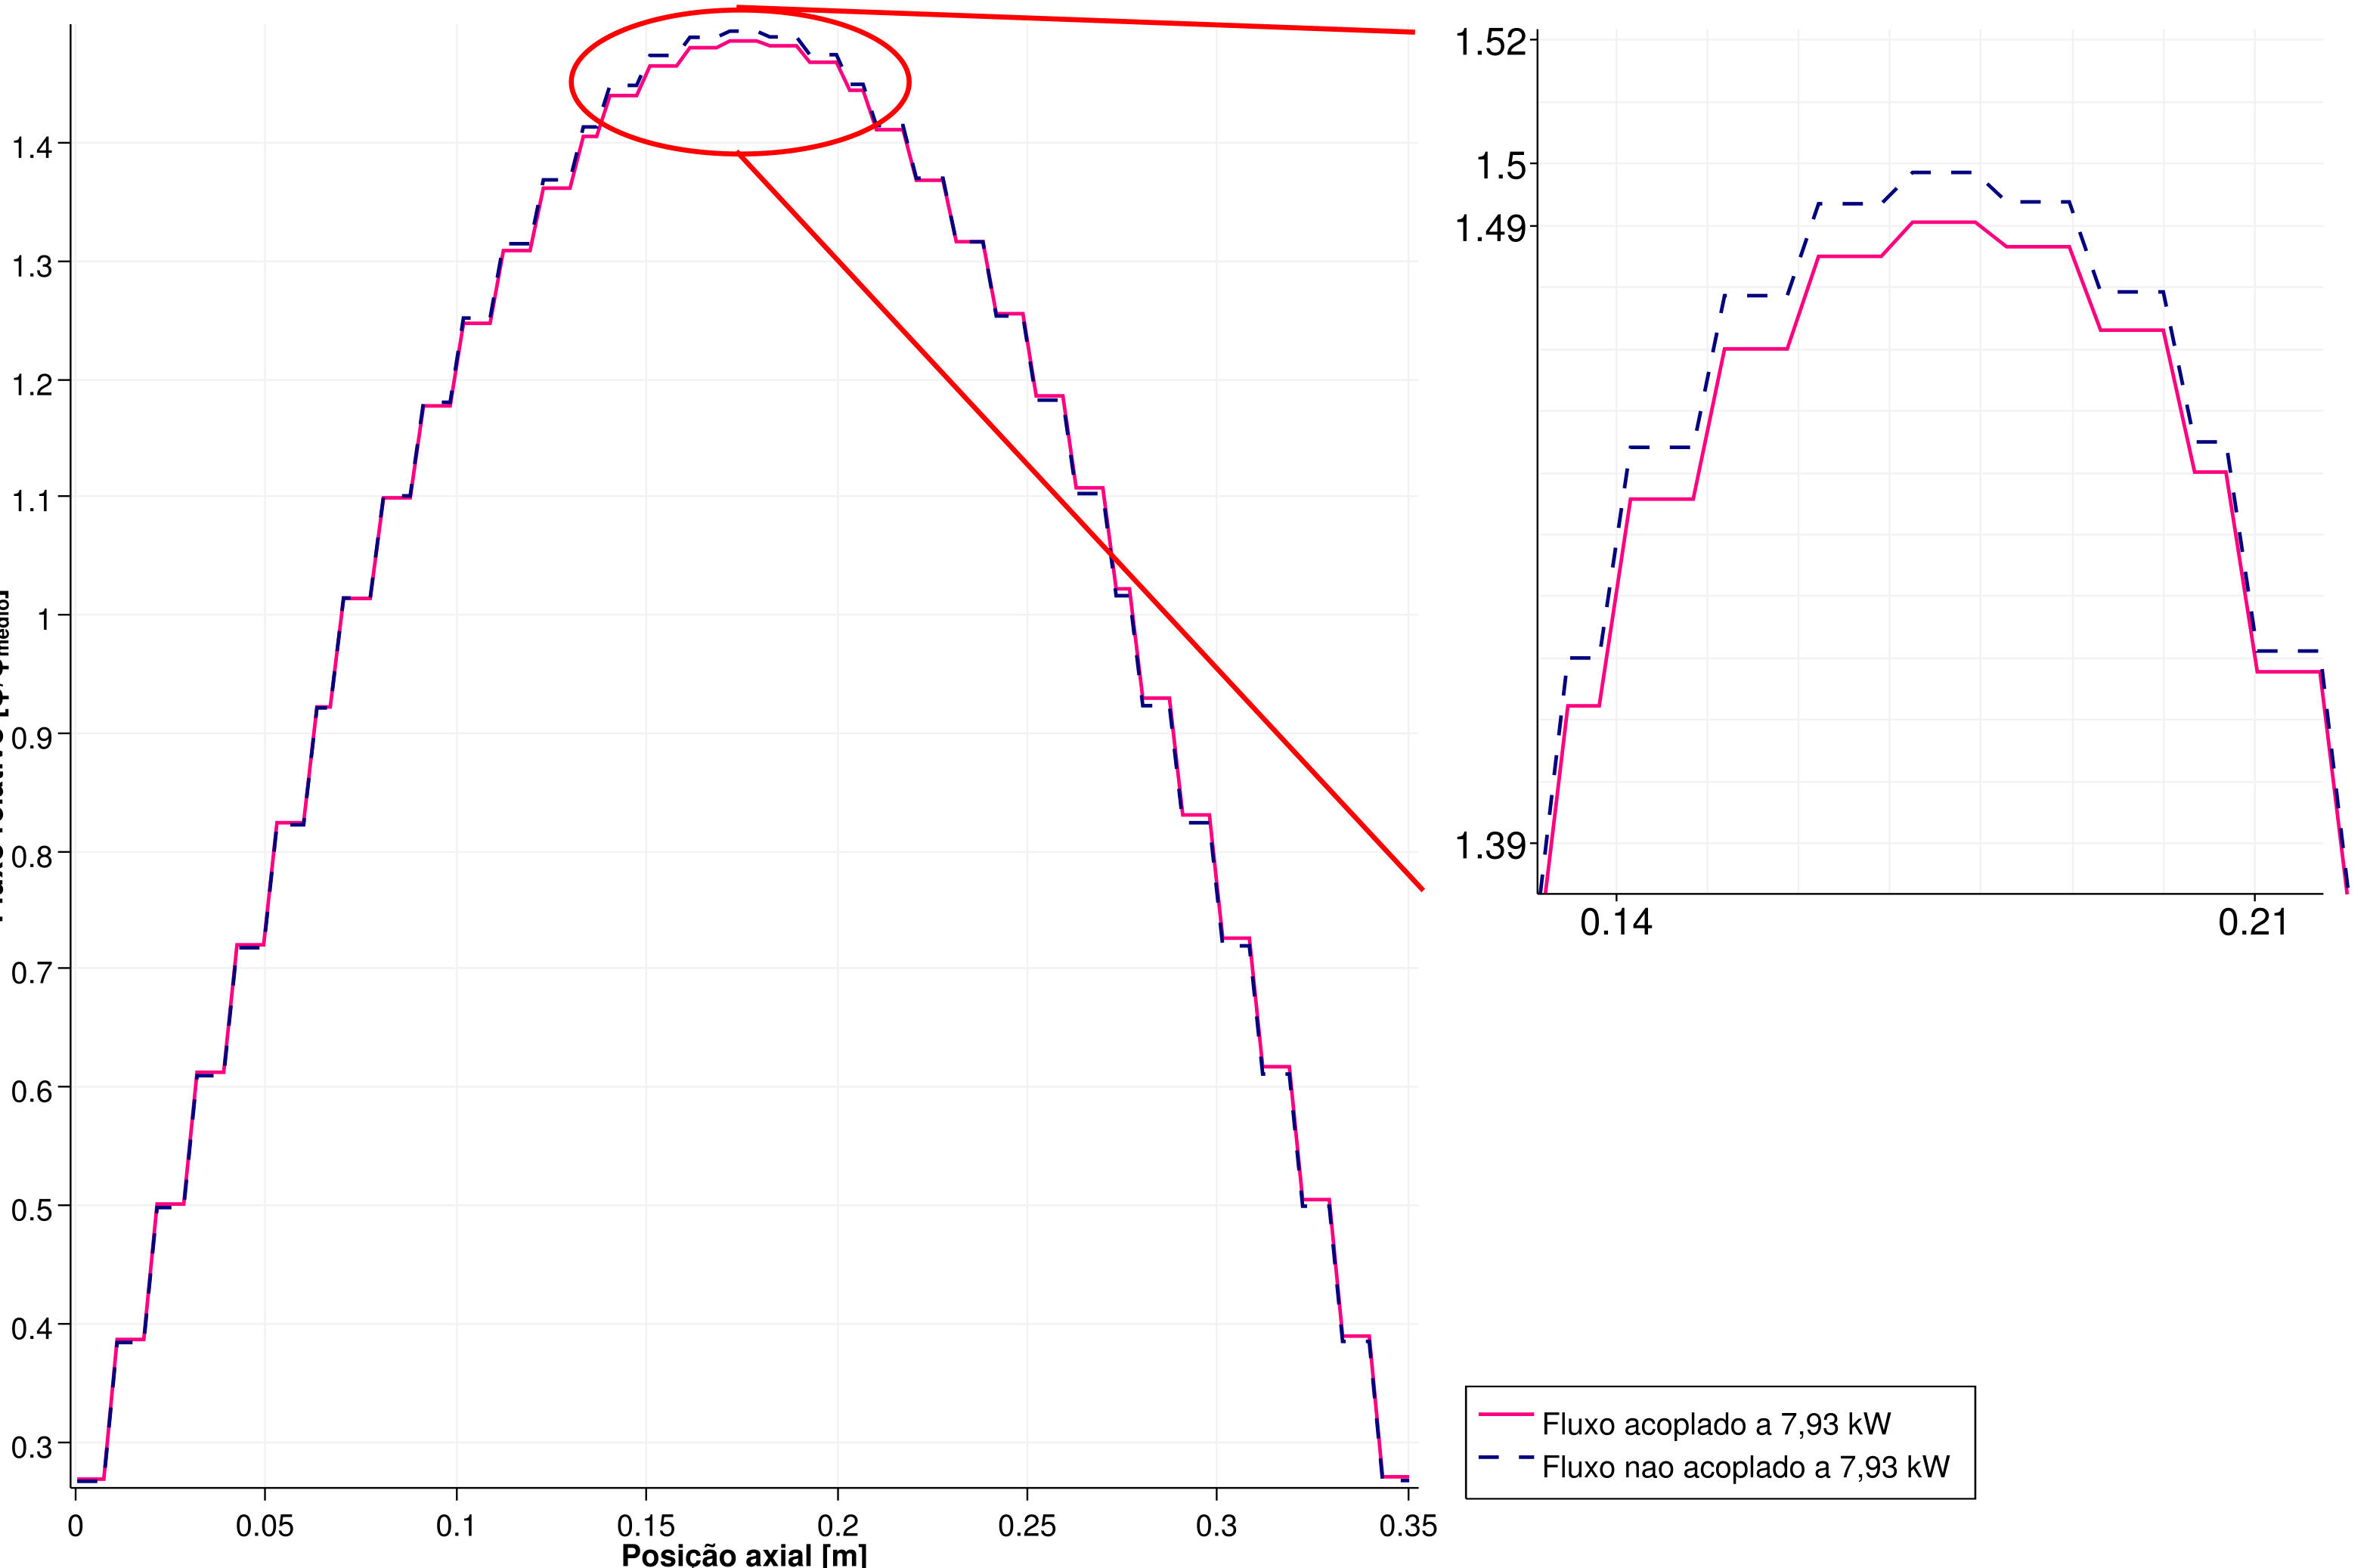
\includegraphics[scale=0.5]{figuras/Flux_rel_z_200_port_trabalhado.png}
  \label{fig:flux_z_200}
%  \legend{Fonte: autor}
\end{figure}

\begin{figure}[htb]
  \caption{Fluxos relativos radiais entre simulação acoplada e não acoplada para
    potência de 7,93 kW.}
  \centering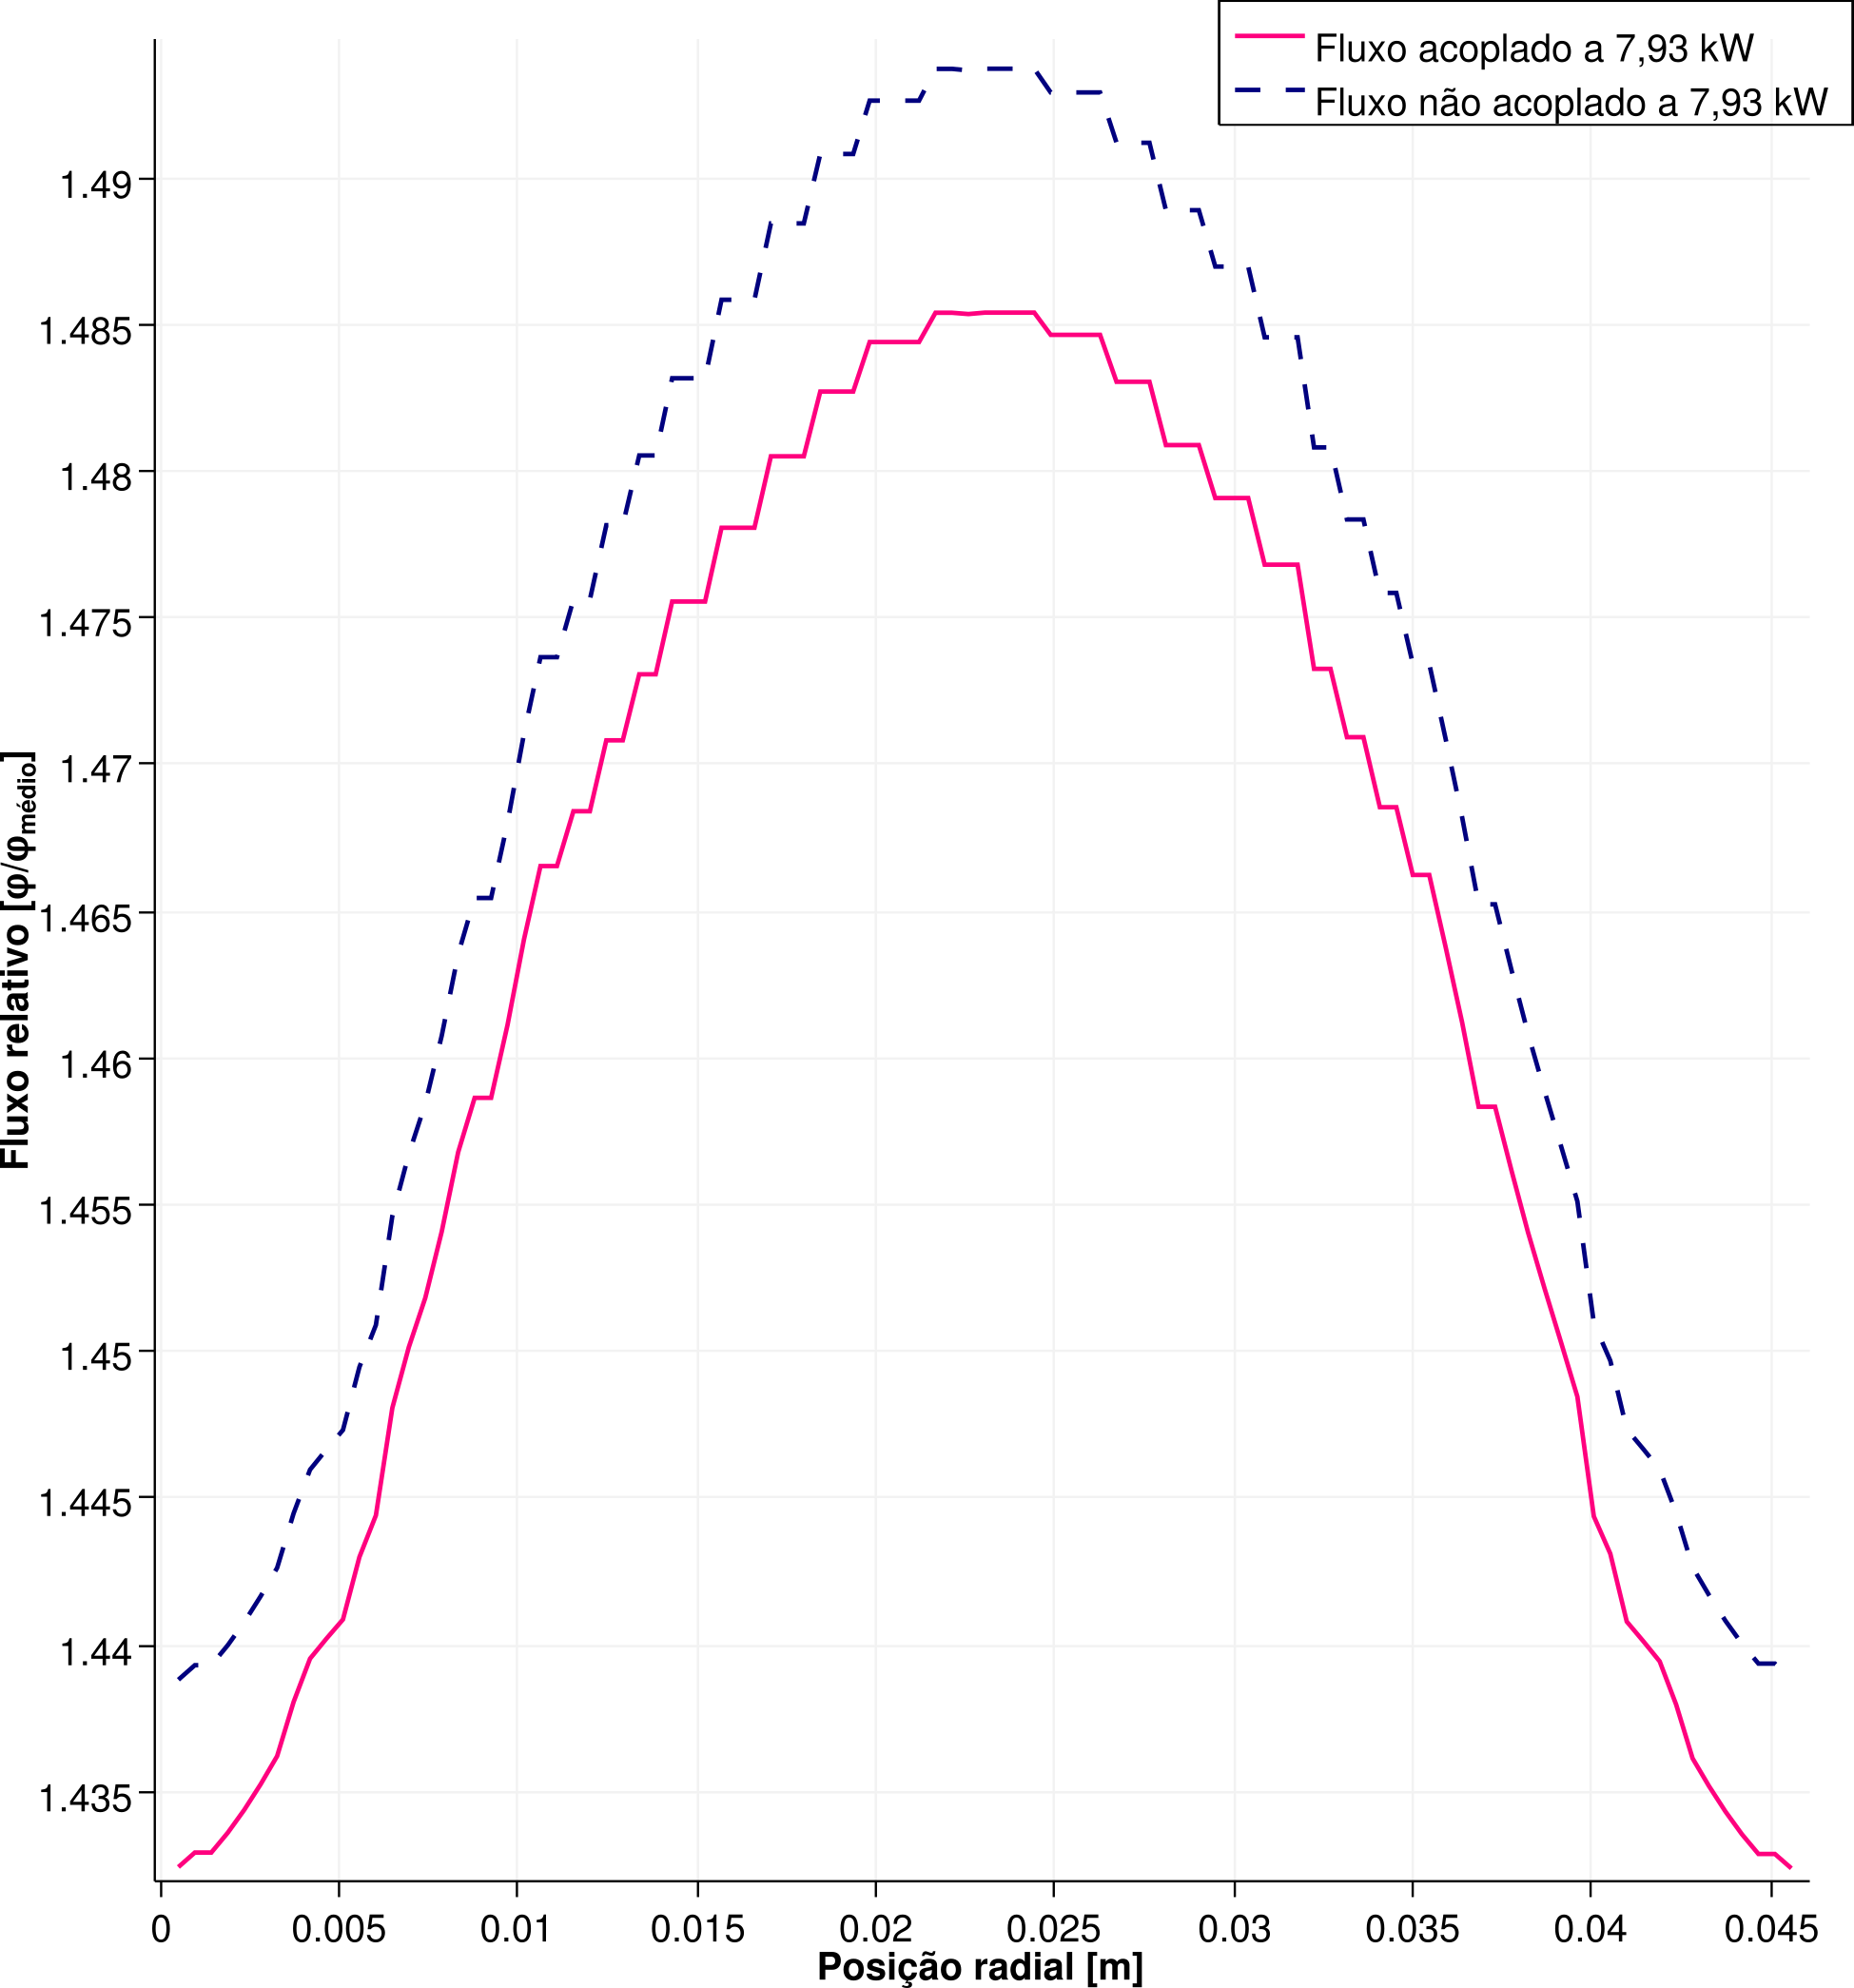
\includegraphics[scale=0.5]{figuras/Flux_rel_x_200_port.png}
  \label{fig:flux_x_200}
%  \legend{Fonte: autor}
\end{figure}

Os perfis de potência para os cálculos acoplados e não-acoplados seguem, como
é de se esperar, o padrão de comportamento dos perfis de fluxo. A solução da
equação de difusão é o fluxo neutrônico e, a partir
dele, é calculada a potência volumétrica baseada em um valor de referência para
a potência.

É a potência
\footnote{A palavra potência é indistintamente utilizada neste capítulo como potência
  propriamente dita, em $W$ ou como sinônimo de densidade de potência, dada em $W/m^3$, de acordo
  com o contexto em que é usada.}
, que entra como termo fonte na equação na energia
resolvida pela termo-hidráulica, que leva ao aquecimento dos materiais que, por sua vez, impactam
no cálculos de seções de choque. As diferenças entre os perfis de potência obtidos nos dois conjuntos
de simulações, acopladas e não-acopladas, são apresentados nas Figuras \ref{fig:Q_all_z} e
\ref{fig:Q_all_x}, respectivamente nas direções axial e radial. Observando estas Figuras,
é possível perceber que as diferenças entre os casos acoplados e
não acoplados aumenta de acordo com o aumento da potência.

Além da diferença em valores absolutos - sutil, para potências mais baixas - entre as curvas obtidas pelos
cálculos acoplados e não acoplados, é possível observar uma mudança no formato das curvas. O perfil de
potência para o cálculo acoplado tem um pico abaixo do pico da simulação
não acoplada, enquanto nas extremidades da curva, os perfis estão sobrepostos\footnote{Na posição
  axial esta diferença não é visível sem aproximação. A diferença em potência é da ordem de dezenas de $kW/m^3$ para medidas da
  ordem de $10^7 kW/m^3$. Para a maior potência simulada, o perfil acoplado está acima nas extremidades.} (Figura \ref{fig:Q_all_z}).

A referida diferença no formato das curvas referentes às simulações acopladas e não acopladas é melhor vista no
perfil radial de potências, Figura \ref{fig:Q_all_x}. O fenômeno ocorre para todas as potências, mas é melhor
visto para a potência de $7,93 kW$. É possível perceber que nos picos, que correspondem à interface entre o
revestimento e o combustível, os valores para a simulação acoplada são maiores. No centro do combustível
ocorre o inverso, sendo menores os valores de potência para a simulação acoplada. Isso se dá devido à realimentação
regular da neutrônica pela temperatura em cada posição. Com o aumento progressivo da temperatura, a reatividade
cai no centro do combustível, levando também a uma diminuição da potência local. Já, nas extremidades, a moderação
de nêutrons que ocorre na água, mais próxima dessa região, leva a mais fissões nessa região. O aumento de temperatura
causado por este aumento na potência é compensado pelo efeito de troca de calor com o revestimento, que está em contato com fluido
a temperaturas mais baixas. Este comportamento é o mesmo que o descrito por Ravnik \cite{Ravnik1990}
para combustíveis do tipo TRIGA, tal qual apresentado anteriormente para o fluxo de nêutrons.

\begin{figure}[htb]
  \caption{Curvas de potência axiais para os casos acoplados e não acoplados.}
  \centering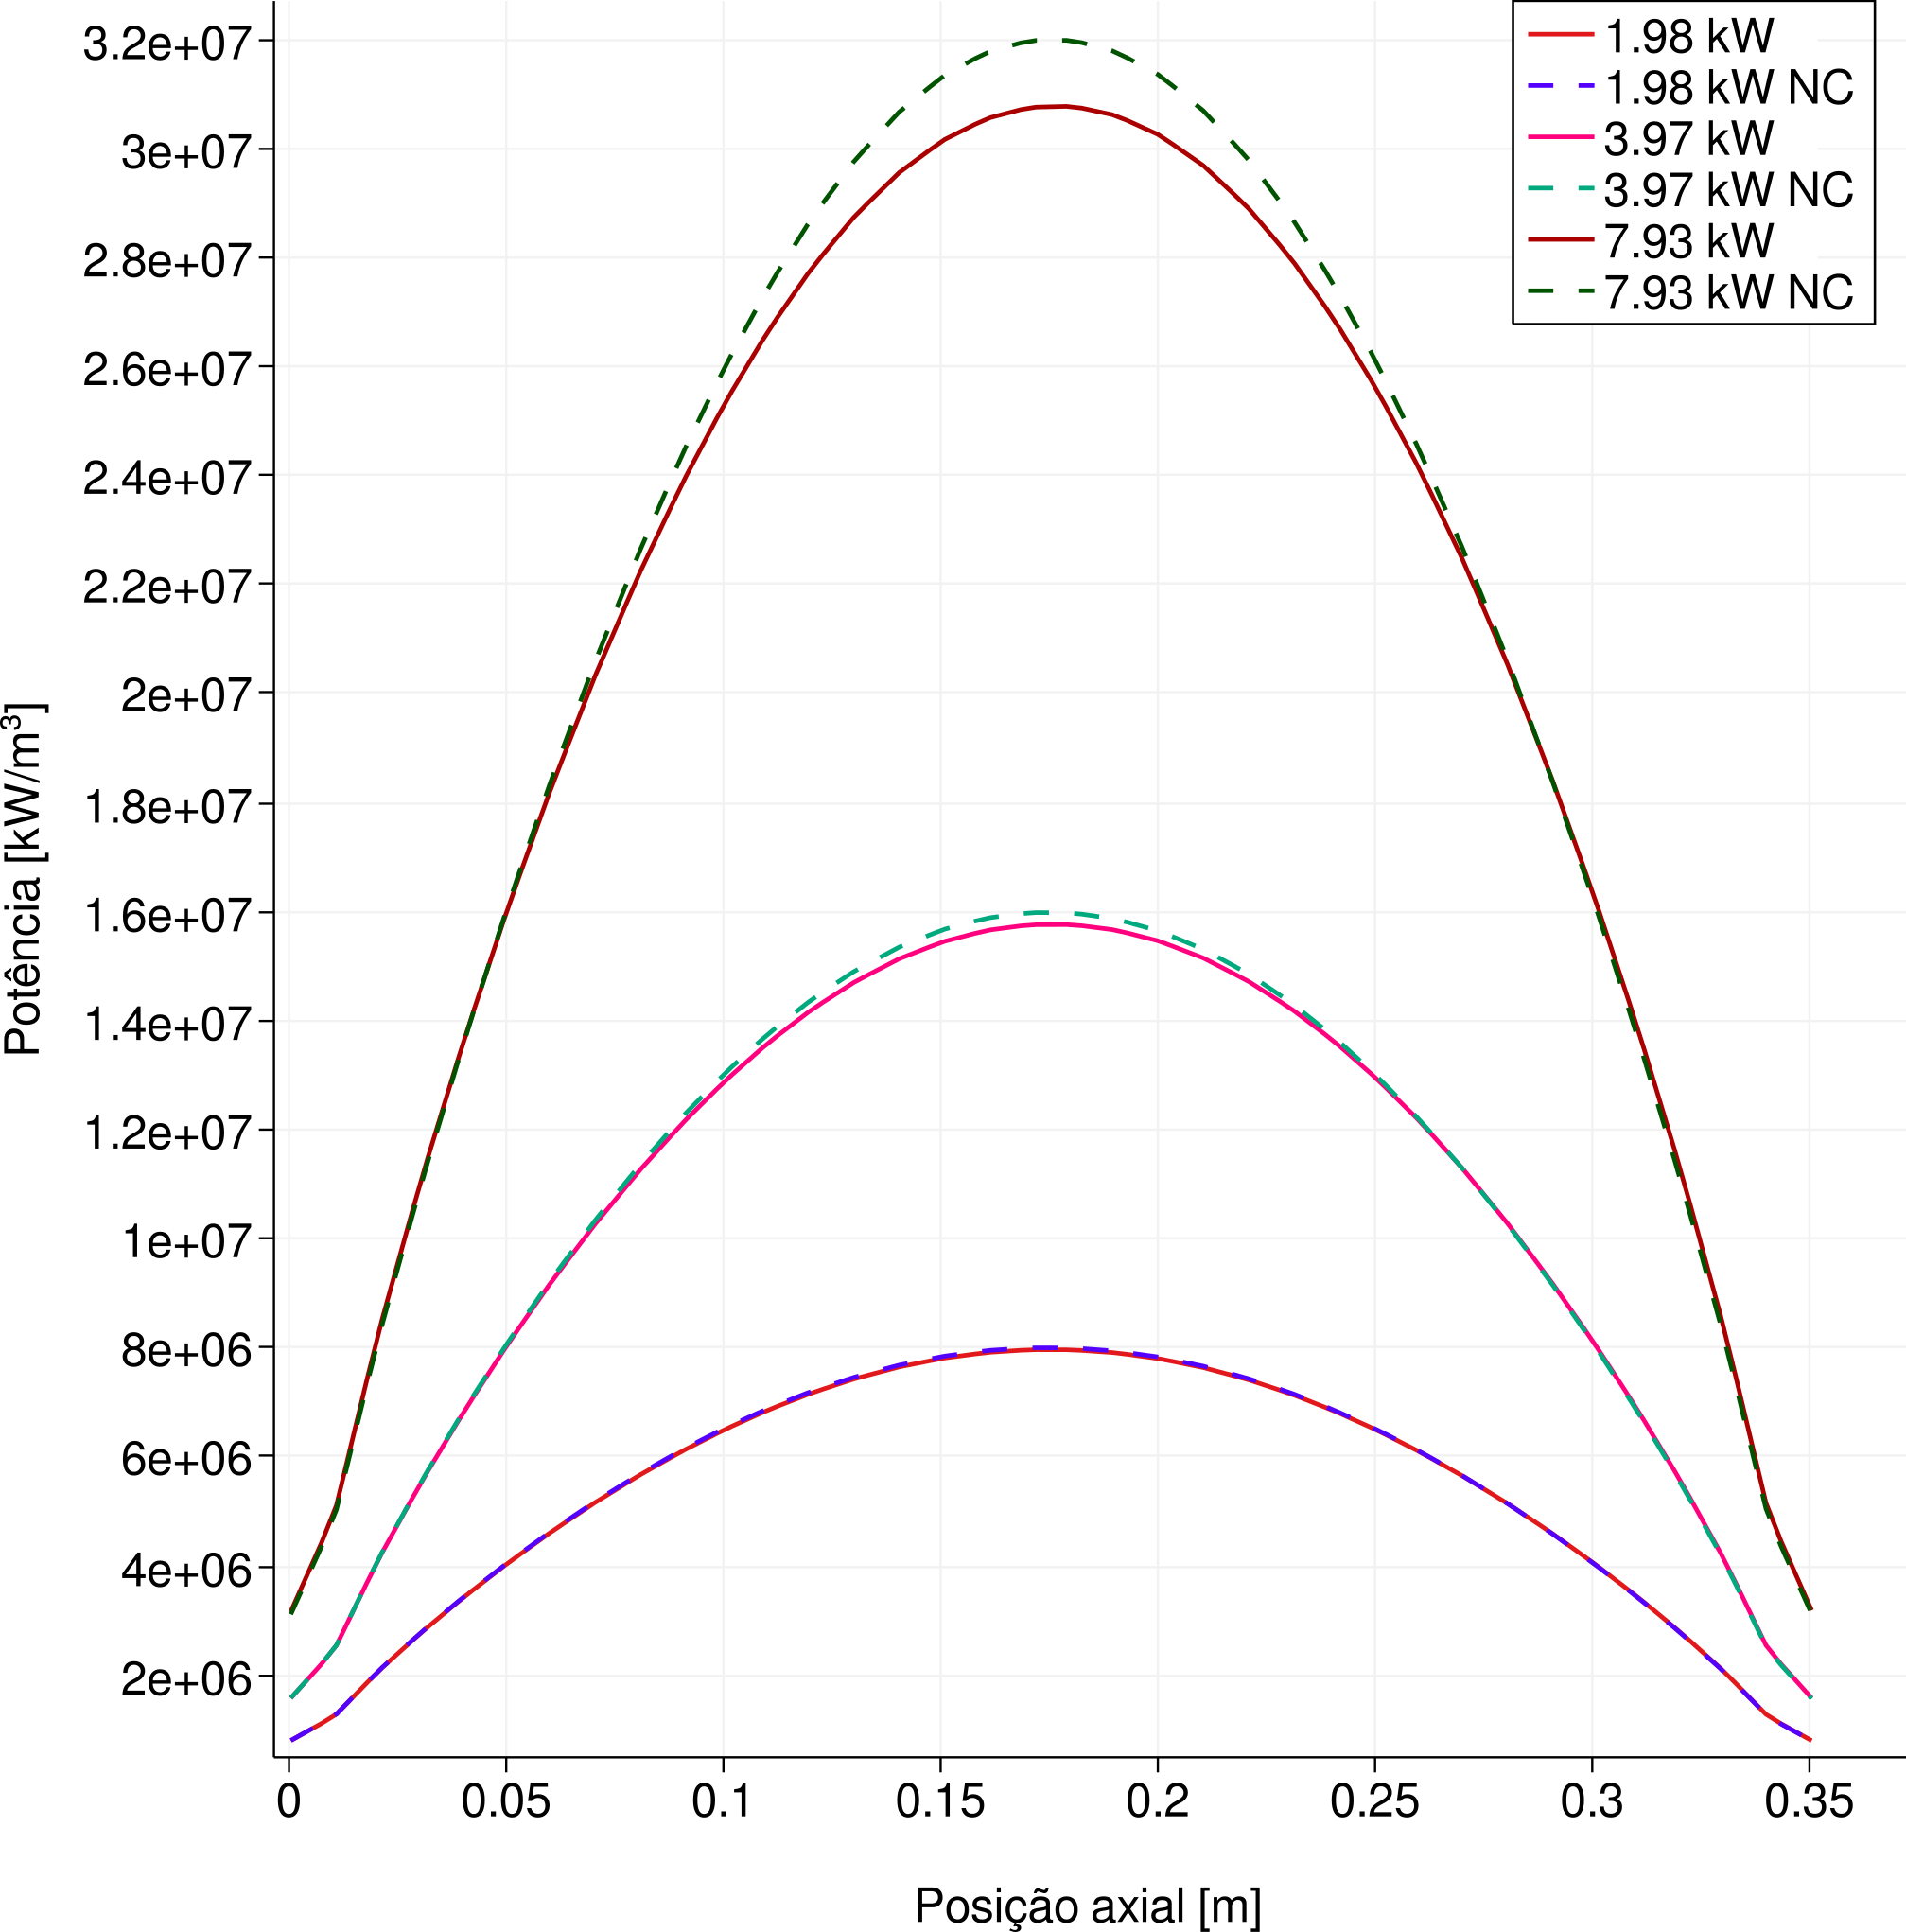
\includegraphics[scale=0.5]{figuras/Q_all_z_square_port.png}
  \label{fig:Q_all_z}
%  \legend{Fonte: autor}
\end{figure}

\begin{figure}[htb]
  \caption{Curvas de potência radiais para os casos acoplados e não acoplados.}
  \centering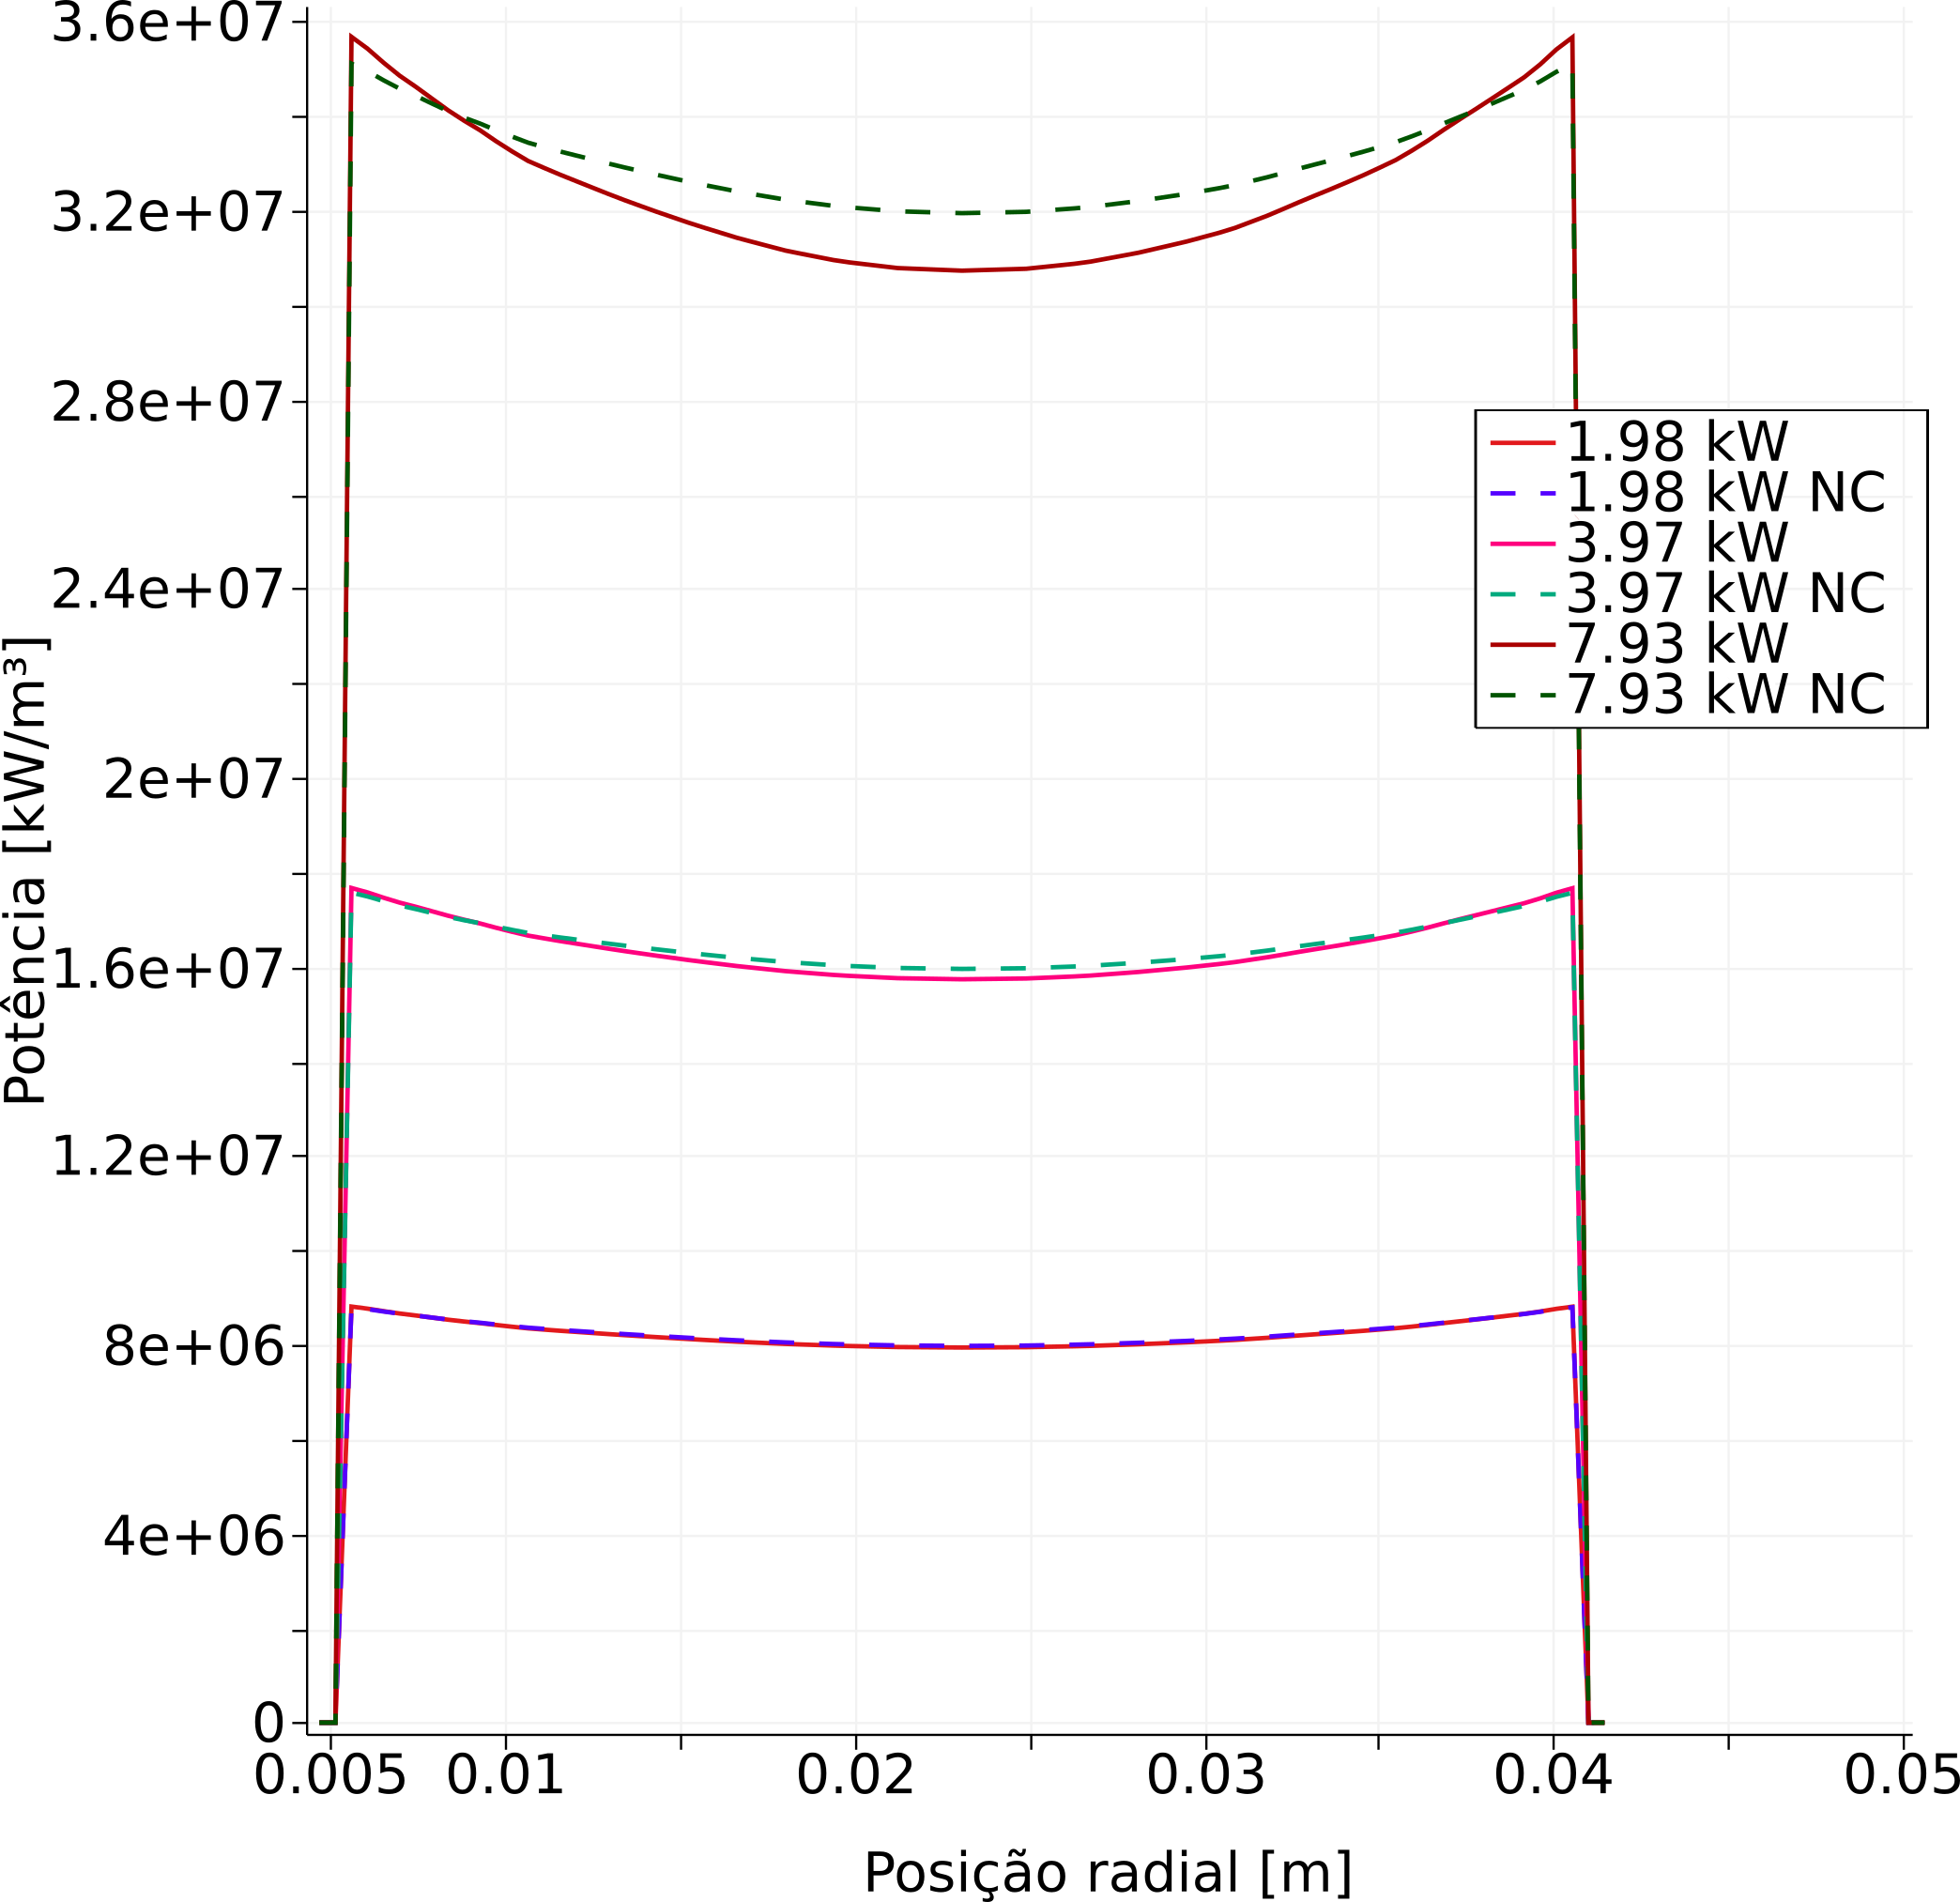
\includegraphics[scale=0.5]{figuras/Q_all_x_square_port.png}
  \label{fig:Q_all_x}
%  \legend{Fonte: autor}
\end{figure}

As curvas de temperaturas para as mesmas simulações são apresentadas nas
Figuras \ref{fig:T_all_z} e \ref{fig:T_all_x}, respectivamente para as
distribuições radial e axial.

As diferenças entre temperaturas para simulações acopladas e não acopladas são
esperadas, uma vez que há variações na distribuição  de potências. As curvas apresentadas nas Figuras
\ref{fig:Q_all_z} e \ref{fig:Q_all_x}, \ref{fig:T_all_z} e \ref{fig:T_all_x} são
as mesmas apresentadas para os casos não acoplados acompanhadas das curvas do
caso acoplado. Os fenômenos físicos e suas explicações para o formato das curvas
são os mesmos, já que as simulações são iguais a menos das potências e do fato
de serem ou não acopladas.

O representativo destes resultados em relação a esta tese está nas diferenças,
pequenas em casos de baixa potência, entre as curvas acopladas e não acopladas.
Em suma, com a retroalimentação devida ao acoplamento, a relação entre os fenômenos
físicos termo-hidráulicos e neutrônicos é representada e, como apresentado,
gera resultados diferentes dos cálculos realizados separadamente.

\begin{figure}[htb]
  \caption{Curvas de temperatura axiais para os casos acoplados e não acoplados.}
  \centering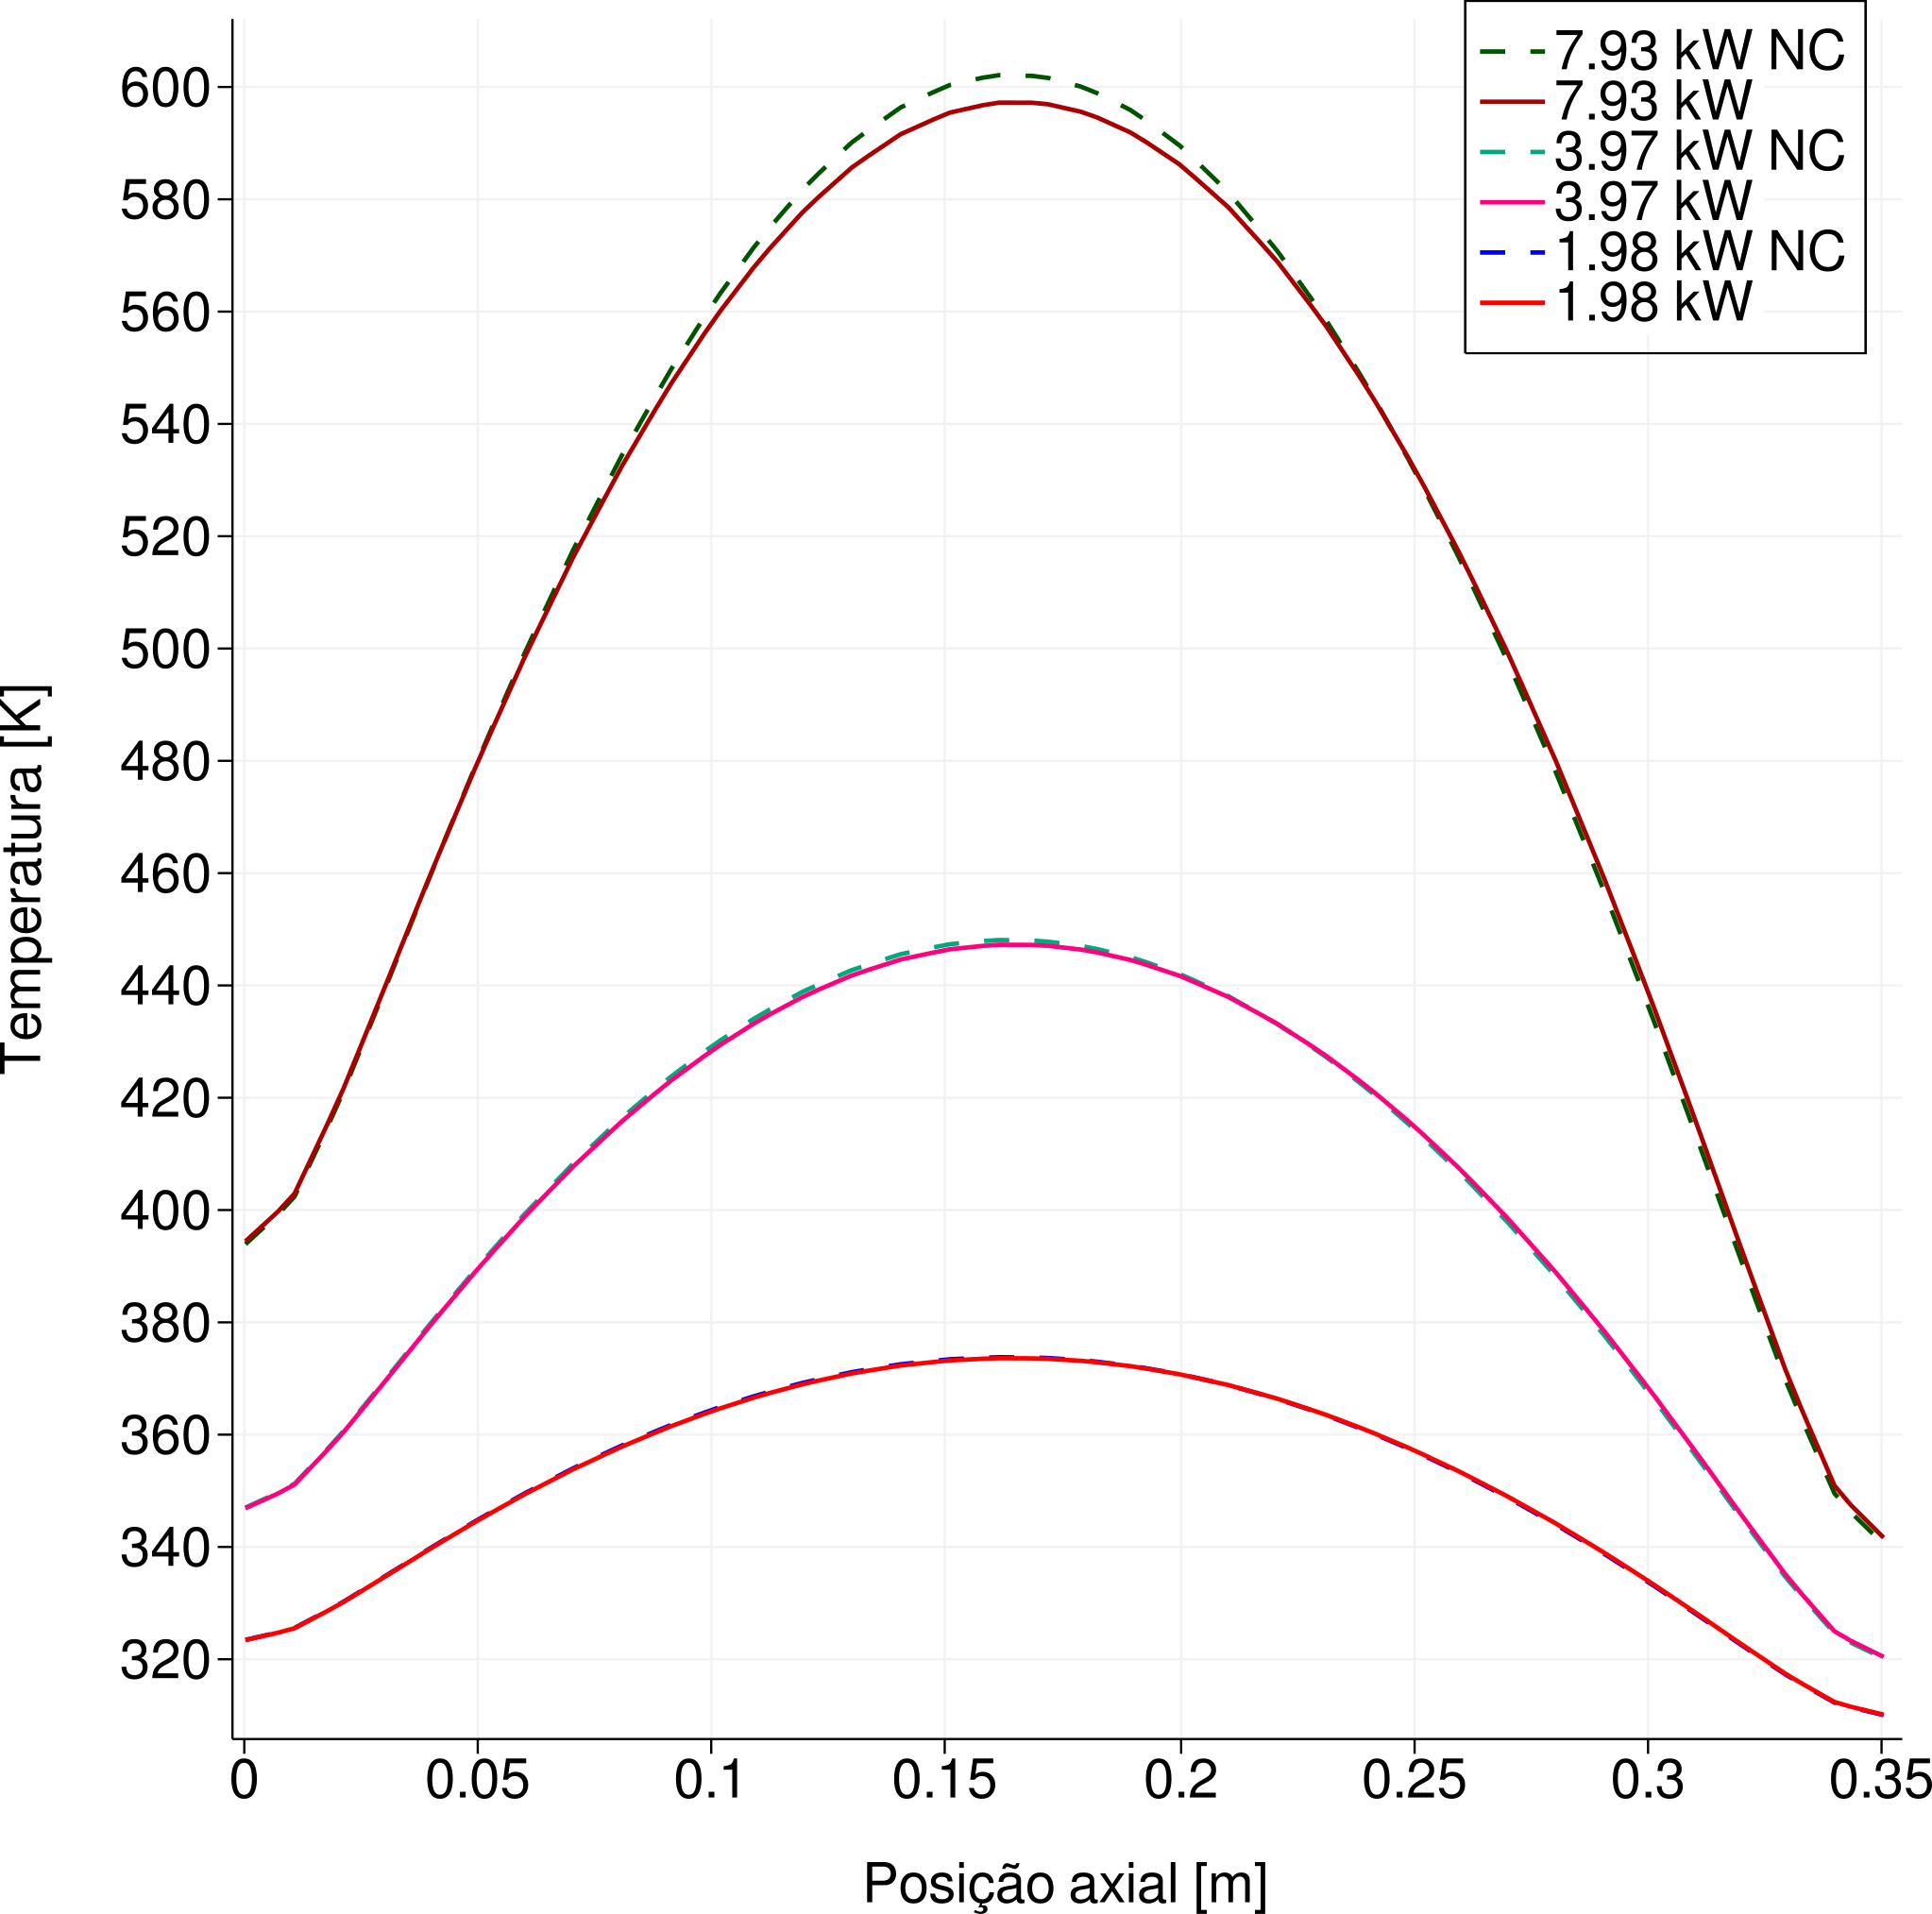
\includegraphics[scale=0.5]{figuras/T_z_all_square_port.png}
  \label{fig:T_all_z}
%  \legend{Fonte: autor}
\end{figure}

\begin{figure}[htb]
  \caption{Curvas de temperatura axiais para os casos acoplados e não acoplados.}
  \centering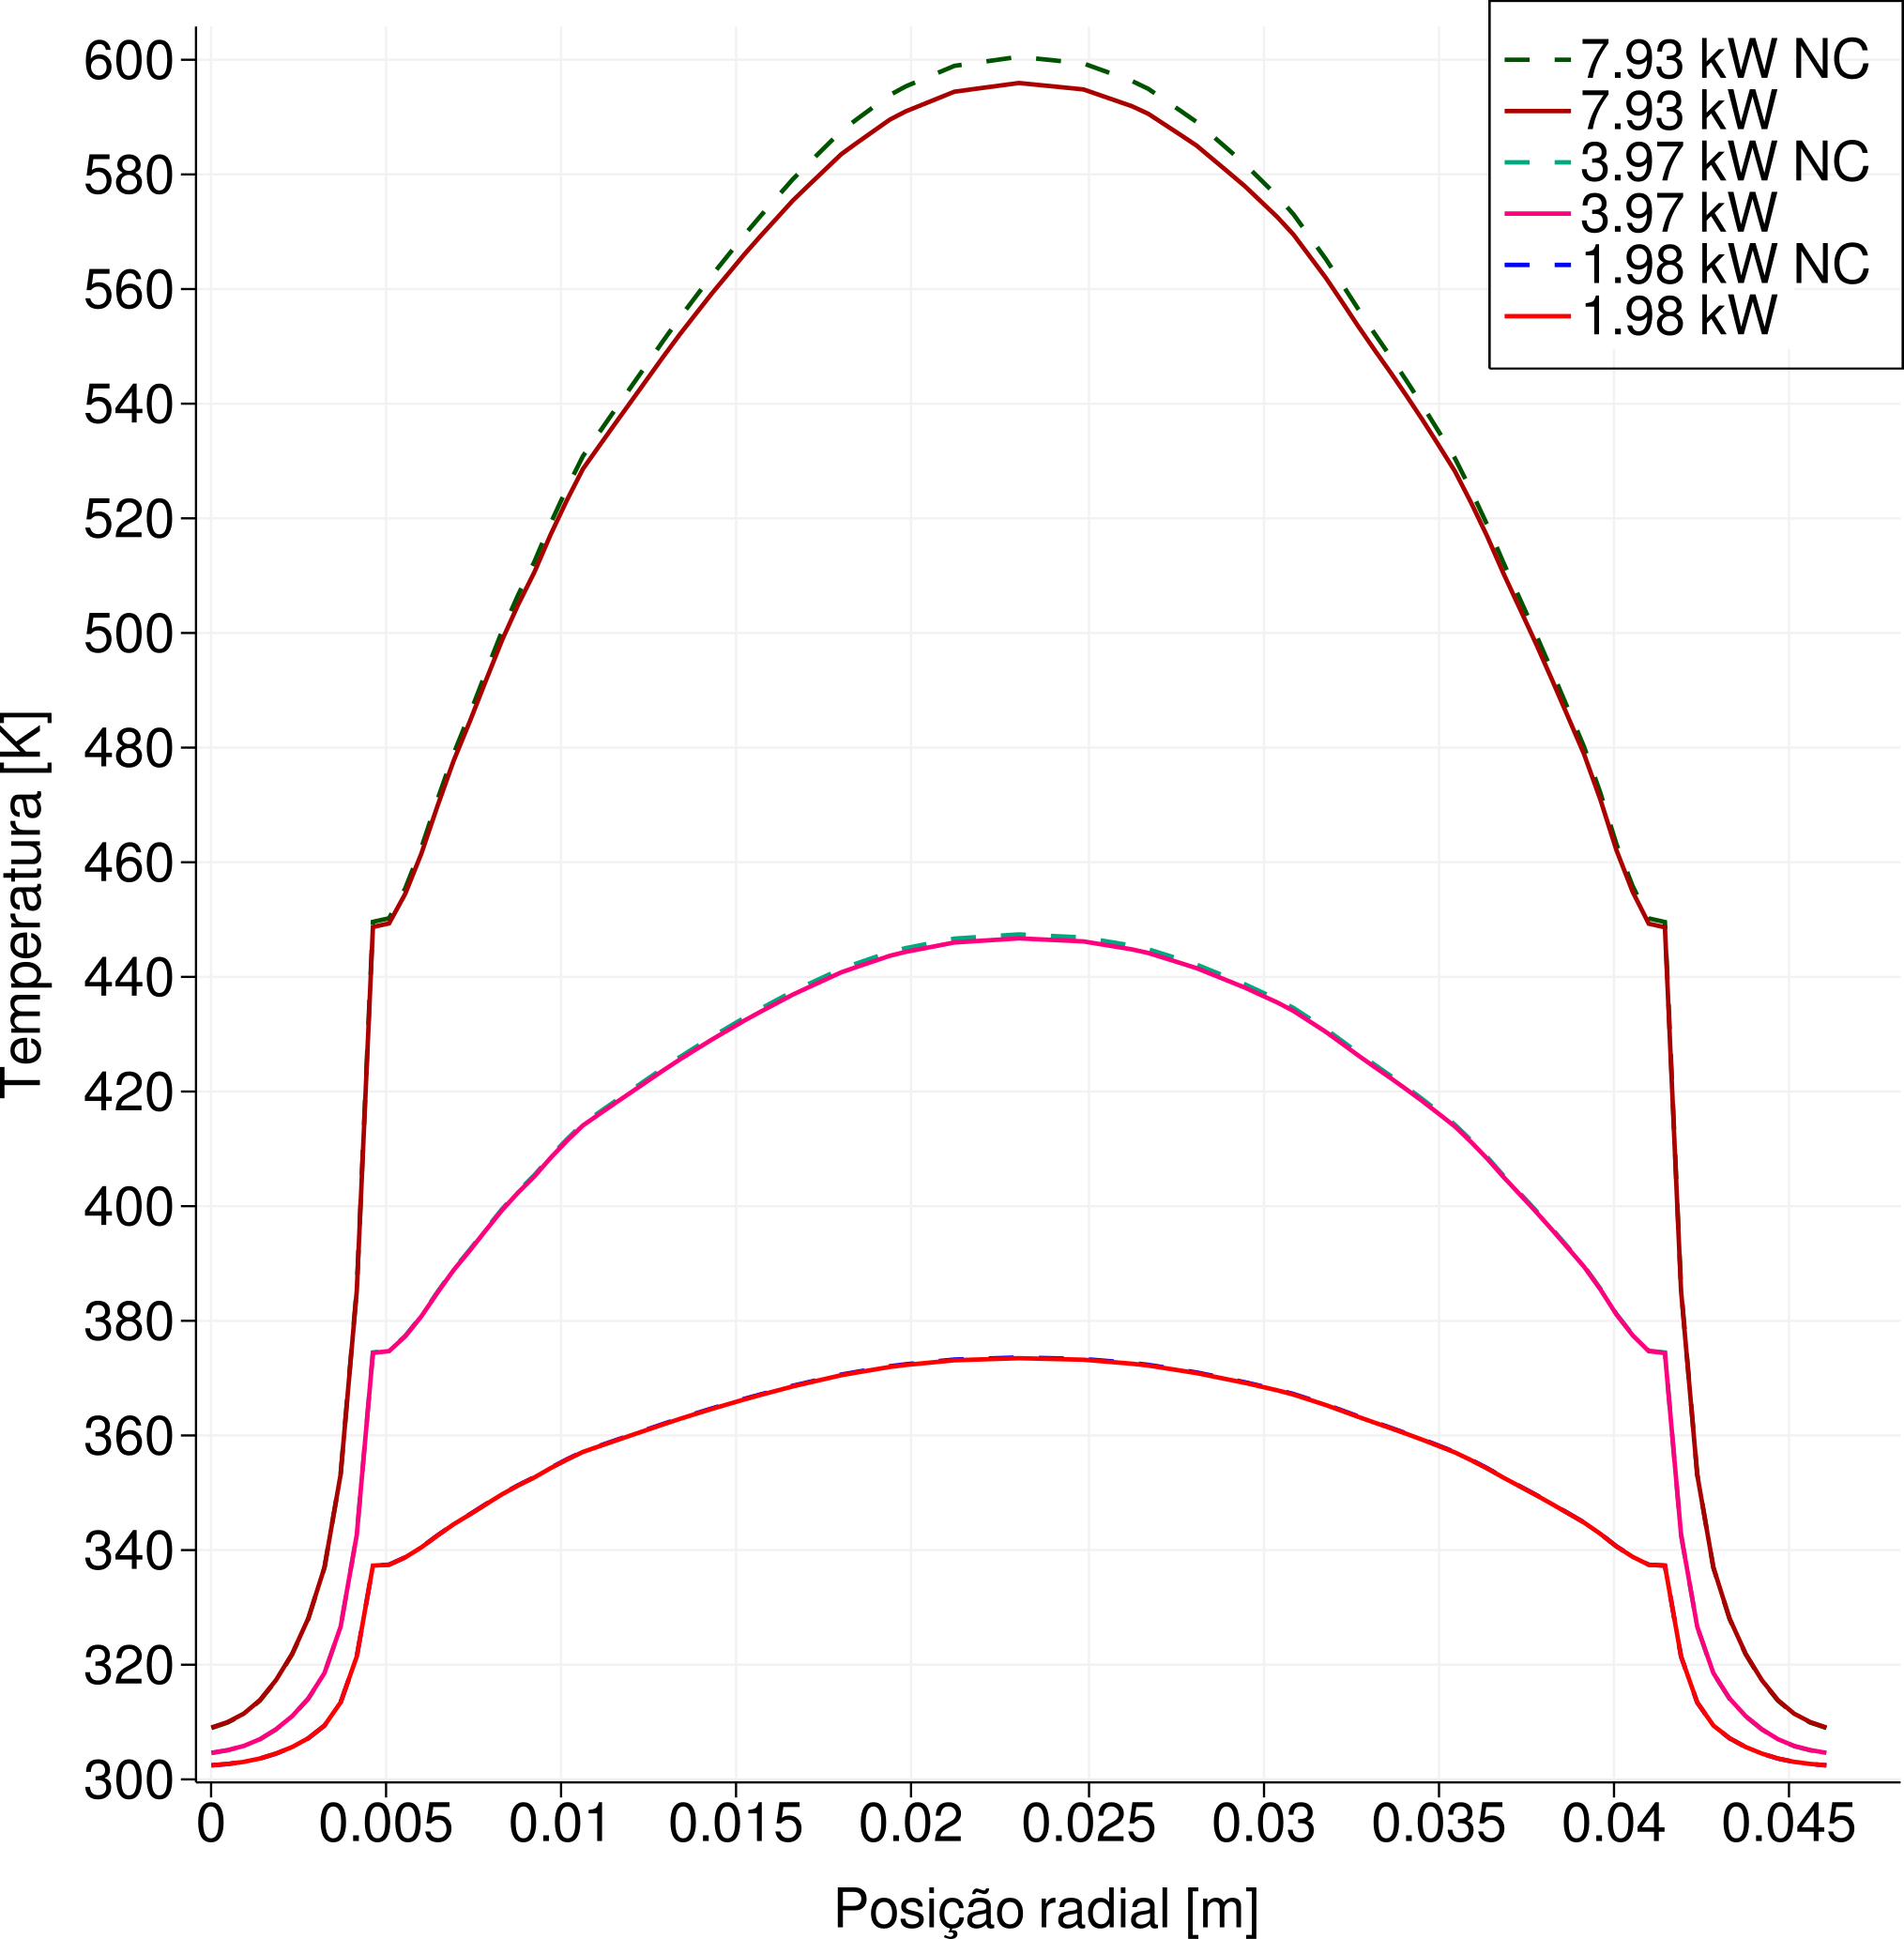
\includegraphics[scale=0.5]{figuras/T_x_all_square_port.png}
  \label{fig:T_all_x}
%  \legend{Fonte: autor}
\end{figure}

Nos cálculos acoplados, a cada execução do \textit{milonga} são utilizadas
novas seções de choque ajustadas a partir de tabelas previamente geradas e da interpolação
destes dados em função das temperaturas de cada célula. Em cada uma destas
execuções, além do fluxo neutrônico, são calculados os fatores de multiplicação
($k_{eff}$) efetivos daquele, digamos, ``estado'' do sistema.

\begin{figure}[htb]
  \caption{Variação dos fatores de multiplicação efetivo ($k_{eff}$) nas três simulações acopladas.}
  \centering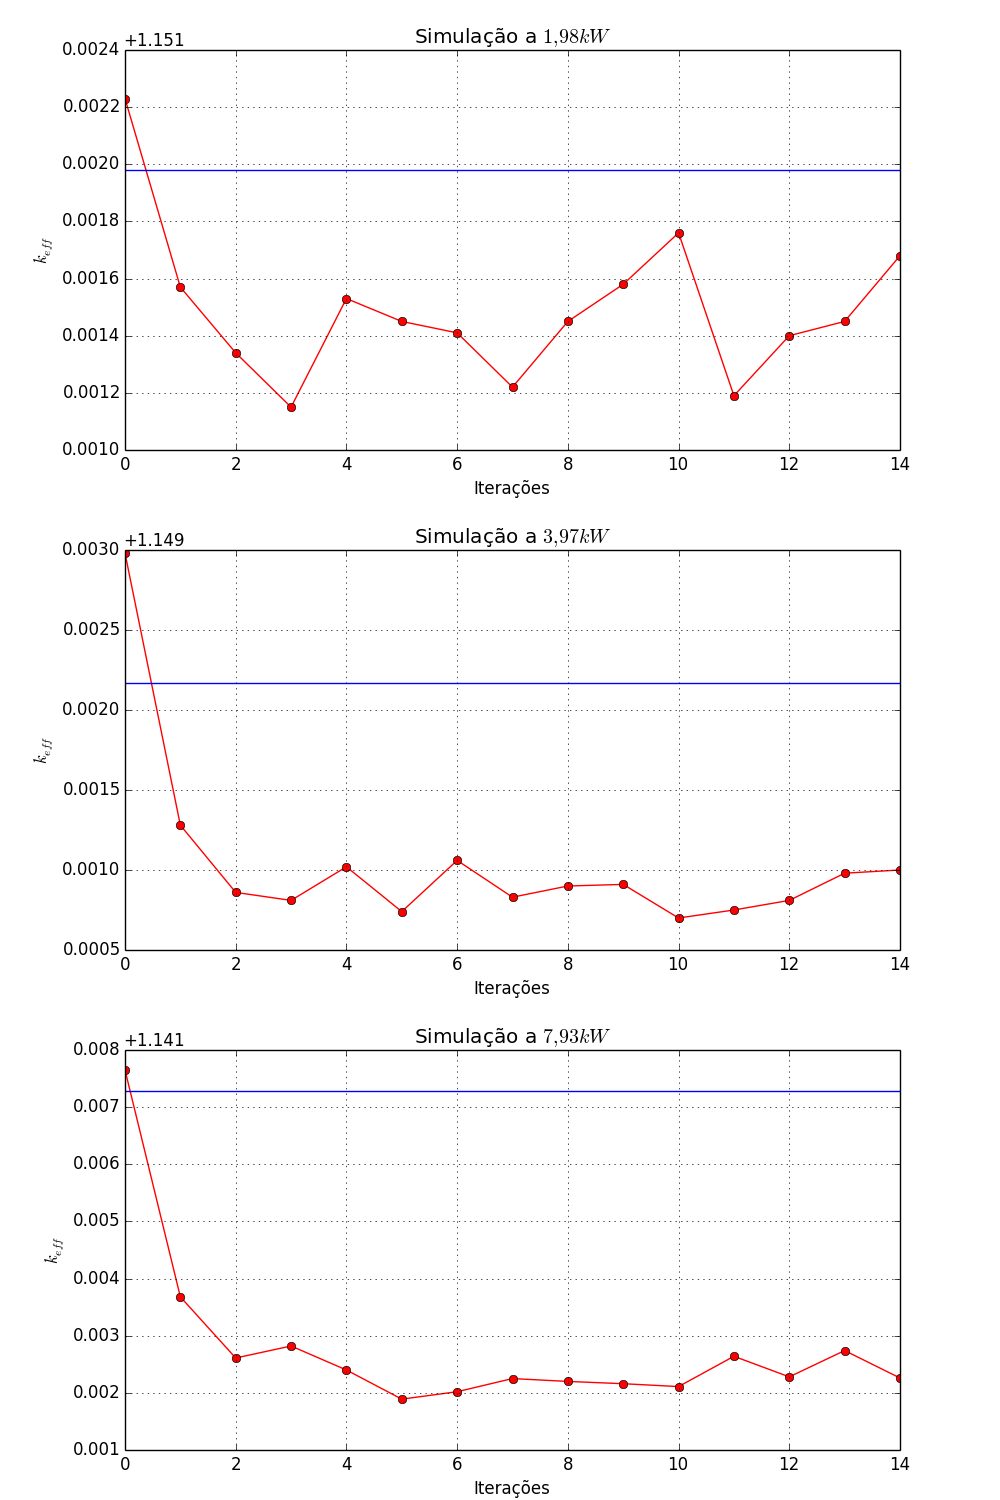
\includegraphics[scale=0.5]{figuras/plot-vertical.png}
  \label{fig:keff_all}
%  \legend{Fonte: autor}
\end{figure}

À medida em que as iterações com o \textit{milonga} ocorrem, o fator de multiplicação
calculado para o sistema varia, oscilando. Esta oscilação ocorre devido à iteração
entre o sistema neutrônico e termo-hidráulico. Intuitivamente, percebe-se que a partir
de uma potência, as temperaturas aumentam na interação seguinte, que leva, por sua vez,
a uma diminuição na reatividade (propriedade deste tipo de elemento combustível),
que leva a uma diminuição na potência, que faz variar a temperatura, que afeta
a reatividade e assim por diante. O fim da simulação se dá por número fixo
de iterações.

Na Figura \ref{fig:keff_all} estão apresentados três gráficos, um para cada simulação
acoplada. As linhas constantes (em azul) indicam o valor do fator de multiplicação
calculado na execução separada do \textit{milonga} com o conjunto inicial de seções
de choque utilizadas no cálculo acoplado. As curvas em vermelho apresentam os fatores
de multiplicação obtidos a cada iteração entre termo-hidráulica e neutrônica (as linhas
entre pontos são apenas para indicação da diferença entre iterações seguidas, já
que os resultados são discretos).

É possível ver que, em todos os casos, os fator de multiplicação cai imediatamente
já após a segunda iteração com a neutrônica. Na primeira iteração entre a
termo-hidráulica e a neutrônica, as temperaturas do sistema vêm subindo devido
à distribuição de potências previamente calculada. A partir desta primeira iteração,
a realimentação do campo de potências já impacta na distribuição de temperaturas,
o que fica claro na segunda iteração. A partir deste ponto, o sistema começa a
apresentar pequenas oscilações ao redor de um fator de multiplicação de convergência.

% ----------------------------------------------------------------------------------
%
% Gráfico de 7,93 em duas simulações. Convergência mais lenta
%
%

Foi realizada, ainda, outra simulação acoplada à potência de $7,93 kW$.
Desta vez, com mudanças nos parâmetros de relaxação para a solução
da equação de energia no sólido que representa o combustível.

Os resultados desta simulação são apresentados no gráfico da Figura \ref{fig:keff_dist}.
Esta simulação necessitou de número maior de iterações que as simulações anteriores para
atingir a convergência. Em outras palavras, foi utilizado inicialmente um parâmetro
mais conservador para a relaxação. Fazendo uso da funcionalidade do \textit{OpenFOAM}
que permite o ajuste de parâmetros de simulação em tempo de execução, tais como
valores de resíduos, mudança de \textit{timestep}, fatores de relaxação, dentre
inúmeros outros, foram alterados os valores de relaxação citados com o objetivo
de diminuir o tempo de convergência dos cálculos\footnote{O objetivo desta funcionalidade é permitir que o
usuário controle a simulação tanto em relação ao tempo total mas também
efetuar um ajuste fino, especialmente útil para evitar a divergência dos
resultados devido à oscilações numéricas.}.

Fica visível, entre as iterações 13 e 16, uma variação mais intensa, se comparada
às anteriores, entre o fator de multiplicação entre iterações consecutivas. Após
este intervalor, as variações passam a ser menores entre iterações consecutivas.

No presente caso, as variações na relaxação dos cálculos da equação da energia para
o sólido, permitiram o aumento da velocidade da convergência, ao mesmo tempo mantendo
os resíduos dos cálculos em níveis aceitáveis, evitando assim a divergência do cálculo.
Tal comportamento mostra que alterações paramétricas em tempo de execução não foram
suficientes para perturbar o sistema acoplado, mostrando certa robustez em relação
a mudanças paramétricas.

\begin{figure}[htb]
  \caption[Variação do fator de multiplicação sobe variação de parâmetros de convergência.]{Variação do fator de multiplicação efetivo ($k_{eff}$) para a simulação a $7,93 kW$ com mudanças em parâmetros de convergência.}
  \centering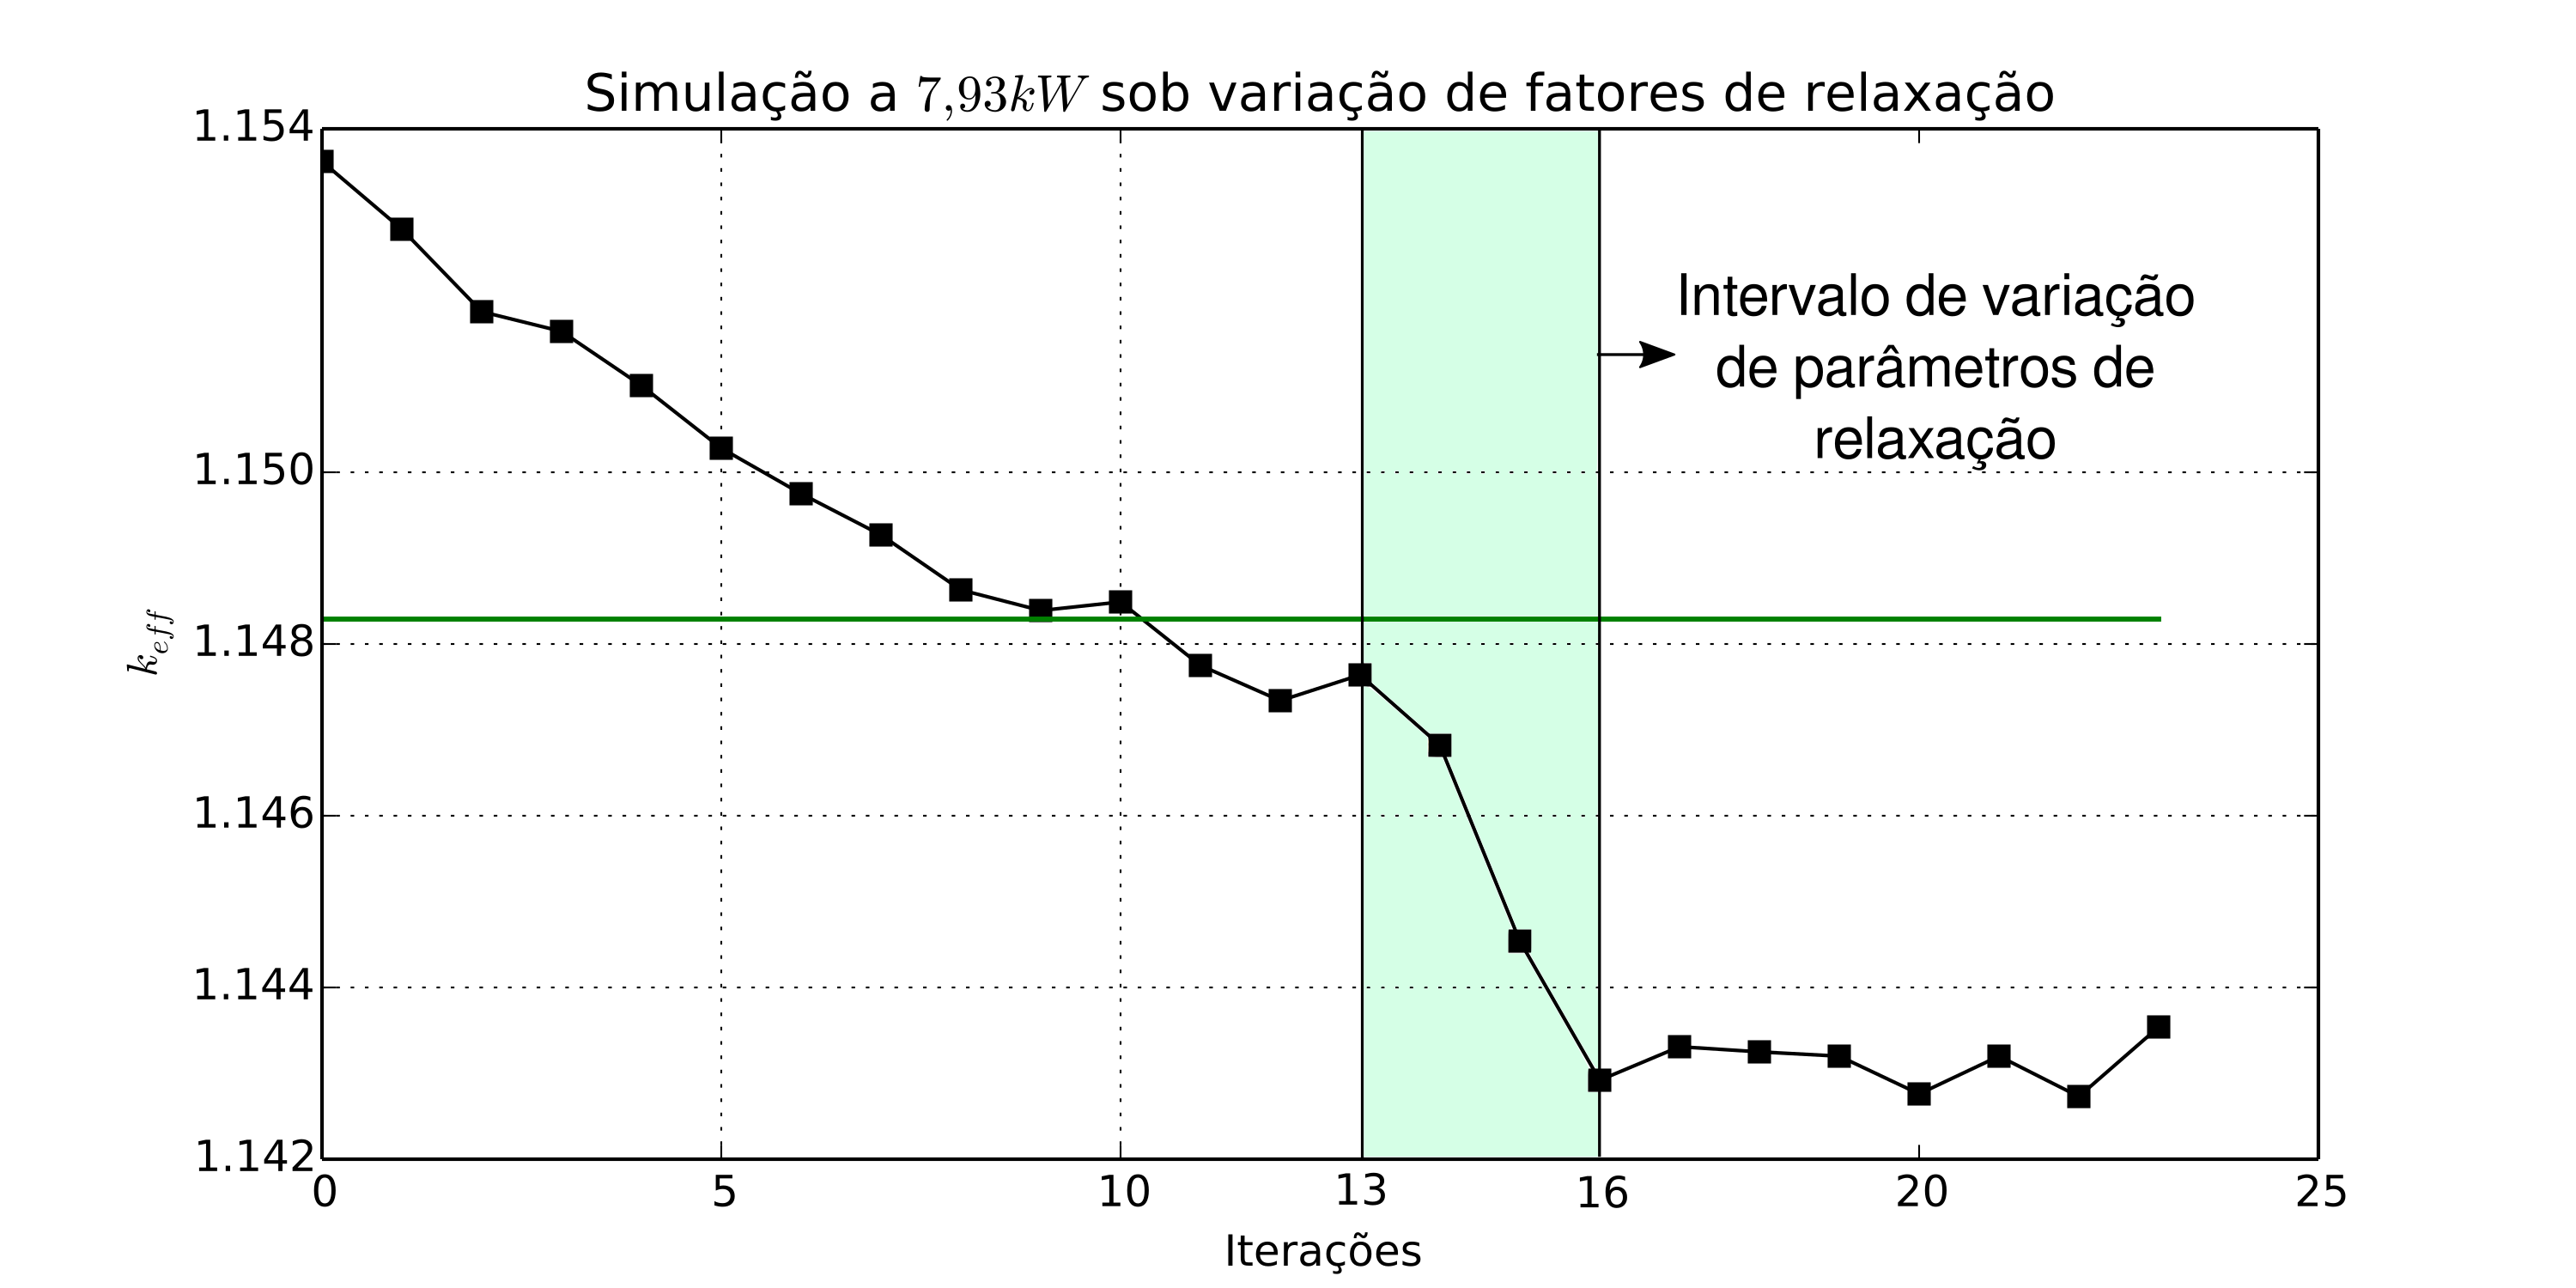
\includegraphics[scale=0.5]{figuras/plot200-disturb-port.png}
  \label{fig:keff_dist}
%  \legend{Fonte: autor}
\end{figure}


Os resultados aqui apresentados não são suficientes para nenhuma afirmação sobre a
efetiva capacidade de cálculos deste sistema acoplado para sistemas mais complexos
do que o modelo utilizado como, por exemplo, uma seção de um núcleo completo de um
reator do tipo TRIGA ou um elemento combustível reduzido de um reator do tipo PWR.
Porém, estes mesmos resultados provam que conceitualmente o acoplamento neutrônico
termo-hidráulico proposto e desenvolvido nesta tese é fisicamente e computacionalmente
consistente, além de funcional.

